% Options for packages loaded elsewhere
\PassOptionsToPackage{unicode}{hyperref}
\PassOptionsToPackage{hyphens}{url}
%
\documentclass[
  english,
  ,man]{apa6}
\usepackage{amsmath,amssymb}
\usepackage{lmodern}
\usepackage{ifxetex,ifluatex}
\ifnum 0\ifxetex 1\fi\ifluatex 1\fi=0 % if pdftex
  \usepackage[T1]{fontenc}
  \usepackage[utf8]{inputenc}
  \usepackage{textcomp} % provide euro and other symbols
\else % if luatex or xetex
  \usepackage{unicode-math}
  \defaultfontfeatures{Scale=MatchLowercase}
  \defaultfontfeatures[\rmfamily]{Ligatures=TeX,Scale=1}
\fi
% Use upquote if available, for straight quotes in verbatim environments
\IfFileExists{upquote.sty}{\usepackage{upquote}}{}
\IfFileExists{microtype.sty}{% use microtype if available
  \usepackage[]{microtype}
  \UseMicrotypeSet[protrusion]{basicmath} % disable protrusion for tt fonts
}{}
\makeatletter
\@ifundefined{KOMAClassName}{% if non-KOMA class
  \IfFileExists{parskip.sty}{%
    \usepackage{parskip}
  }{% else
    \setlength{\parindent}{0pt}
    \setlength{\parskip}{6pt plus 2pt minus 1pt}}
}{% if KOMA class
  \KOMAoptions{parskip=half}}
\makeatother
\usepackage{xcolor}
\IfFileExists{xurl.sty}{\usepackage{xurl}}{} % add URL line breaks if available
\IfFileExists{bookmark.sty}{\usepackage{bookmark}}{\usepackage{hyperref}}
\hypersetup{
  pdftitle={Why Most Studies of Individual Differences With Inhibition Tasks Are Bound To Fail},
  pdfauthor={Jeffrey N. Rouder1, Aakriti Kumar1, \& Julia M. Haaf2},
  pdflang={en-EN},
  pdfkeywords={Individual Differences, Cognitive Tasks, Hierarchical Models, Bayesian Inference},
  hidelinks,
  pdfcreator={LaTeX via pandoc}}
\urlstyle{same} % disable monospaced font for URLs
\usepackage{graphicx}
\makeatletter
\def\maxwidth{\ifdim\Gin@nat@width>\linewidth\linewidth\else\Gin@nat@width\fi}
\def\maxheight{\ifdim\Gin@nat@height>\textheight\textheight\else\Gin@nat@height\fi}
\makeatother
% Scale images if necessary, so that they will not overflow the page
% margins by default, and it is still possible to overwrite the defaults
% using explicit options in \includegraphics[width, height, ...]{}
\setkeys{Gin}{width=\maxwidth,height=\maxheight,keepaspectratio}
% Set default figure placement to htbp
\makeatletter
\def\fps@figure{htbp}
\makeatother
\setlength{\emergencystretch}{3em} % prevent overfull lines
\providecommand{\tightlist}{%
  \setlength{\itemsep}{0pt}\setlength{\parskip}{0pt}}
\setcounter{secnumdepth}{-\maxdimen} % remove section numbering
% Make \paragraph and \subparagraph free-standing
\ifx\paragraph\undefined\else
  \let\oldparagraph\paragraph
  \renewcommand{\paragraph}[1]{\oldparagraph{#1}\mbox{}}
\fi
\ifx\subparagraph\undefined\else
  \let\oldsubparagraph\subparagraph
  \renewcommand{\subparagraph}[1]{\oldsubparagraph{#1}\mbox{}}
\fi
% Manuscript styling
\usepackage{upgreek}
\captionsetup{font=singlespacing,justification=justified}

% Table formatting
\usepackage{longtable}
\usepackage{lscape}
% \usepackage[counterclockwise]{rotating}   % Landscape page setup for large tables
\usepackage{multirow}		% Table styling
\usepackage{tabularx}		% Control Column width
\usepackage[flushleft]{threeparttable}	% Allows for three part tables with a specified notes section
\usepackage{threeparttablex}            % Lets threeparttable work with longtable

% Create new environments so endfloat can handle them
% \newenvironment{ltable}
%   {\begin{landscape}\centering\begin{threeparttable}}
%   {\end{threeparttable}\end{landscape}}
\newenvironment{lltable}{\begin{landscape}\centering\begin{ThreePartTable}}{\end{ThreePartTable}\end{landscape}}

% Enables adjusting longtable caption width to table width
% Solution found at http://golatex.de/longtable-mit-caption-so-breit-wie-die-tabelle-t15767.html
\makeatletter
\newcommand\LastLTentrywidth{1em}
\newlength\longtablewidth
\setlength{\longtablewidth}{1in}
\newcommand{\getlongtablewidth}{\begingroup \ifcsname LT@\roman{LT@tables}\endcsname \global\longtablewidth=0pt \renewcommand{\LT@entry}[2]{\global\advance\longtablewidth by ##2\relax\gdef\LastLTentrywidth{##2}}\@nameuse{LT@\roman{LT@tables}} \fi \endgroup}

% \setlength{\parindent}{0.5in}
% \setlength{\parskip}{0pt plus 0pt minus 0pt}

% \usepackage{etoolbox}
\makeatletter
\patchcmd{\HyOrg@maketitle}
  {\section{\normalfont\normalsize\abstractname}}
  {\section*{\normalfont\normalsize\abstractname}}
  {}{\typeout{Failed to patch abstract.}}
\patchcmd{\HyOrg@maketitle}
  {\section{\protect\normalfont{\@title}}}
  {\section*{\protect\normalfont{\@title}}}
  {}{\typeout{Failed to patch title.}}
\makeatother
\shorttitle{Individual Differences in Cognitive Tasks}
\keywords{Individual Differences, Cognitive Tasks, Hierarchical Models, Bayesian Inference}
\DeclareDelayedFloatFlavor{ThreePartTable}{table}
\DeclareDelayedFloatFlavor{lltable}{table}
\DeclareDelayedFloatFlavor*{longtable}{table}
\makeatletter
\renewcommand{\efloat@iwrite}[1]{\immediate\expandafter\protected@write\csname efloat@post#1\endcsname{}}
\makeatother
\usepackage{csquotes}
\usepackage{bm}
\usepackage{amsmath}
\usepackage{setspace}
\usepackage{pcl}
\usepackage{marginnote}
\newcommand{\readme}[1]{\emph{\marginnote{Julia} (#1)}}
\ifxetex
  % Load polyglossia as late as possible: uses bidi with RTL langages (e.g. Hebrew, Arabic)
  \usepackage{polyglossia}
  \setmainlanguage[]{english}
\else
  \usepackage[main=english]{babel}
% get rid of language-specific shorthands (see #6817):
\let\LanguageShortHands\languageshorthands
\def\languageshorthands#1{}
\fi
\ifluatex
  \usepackage{selnolig}  % disable illegal ligatures
\fi
\newlength{\cslhangindent}
\setlength{\cslhangindent}{1.5em}
\newlength{\csllabelwidth}
\setlength{\csllabelwidth}{3em}
\newenvironment{CSLReferences}[2] % #1 hanging-ident, #2 entry spacing
 {% don't indent paragraphs
  \setlength{\parindent}{0pt}
  % turn on hanging indent if param 1 is 1
  \ifodd #1 \everypar{\setlength{\hangindent}{\cslhangindent}}\ignorespaces\fi
  % set entry spacing
  \ifnum #2 > 0
  \setlength{\parskip}{#2\baselineskip}
  \fi
 }%
 {}
\usepackage{calc}
\newcommand{\CSLBlock}[1]{#1\hfill\break}
\newcommand{\CSLLeftMargin}[1]{\parbox[t]{\csllabelwidth}{#1}}
\newcommand{\CSLRightInline}[1]{\parbox[t]{\linewidth - \csllabelwidth}{#1}\break}
\newcommand{\CSLIndent}[1]{\hspace{\cslhangindent}#1}

\title{Why Most Studies of Individual Differences With Inhibition Tasks Are Bound To Fail}
\author{Jeffrey N. Rouder\textsuperscript{1}, Aakriti Kumar\textsuperscript{1}, \& Julia M. Haaf\textsuperscript{2}}
\date{}


\note{Version 3.0}

\affiliation{\vspace{0.5cm}\textsuperscript{1} University of California, Irvine\\\textsuperscript{2} University of Amsterdam}

\abstract{
Establishing correlations among common inhibition tasks such as Stroop or flanker tasks has been proven quite difficult despite many attempts. It remains unknown whether this difficulty occurs because inhibition is a disparate set of phenomena or whether the analytic techniques to uncover a unified inhibition phenomenon fail in real-world contexts. In this paper, we explore the field-wide inability to assess whether inhibition is unified or disparate. We do so by showing that ordinary methods of correlating performance including those with latent variable models are doomed to fail because of trial noise (or, as it is sometimes called, measurement error). We then develop hierarchical models that account for variation across trials, variation across individuals, and covariation across individuals and tasks. These hierarchical models also fail to uncover correlations in typical designs for the same reasons. While we can characterize the degree of trial noise, we cannot recover correlations in typical designs that enroll hundreds of people. We discuss possible improvements to study designs to help uncovering correlations, though we are not sure how feasible they are.
}



\begin{document}
\maketitle

In 1957, Lee Cronbach gave a presidential address to the American Psychological Association where he advocates merging two major but separate traditions in research psychology (Cronbach, 1957). One was termed the \emph{correlational tradition}, and it referred to the rapid advances in psychometrics and scaling at the time. The other was the \emph{experimental tradition,} which is readily recognizable in this journal and several others. Although these traditions remain largely separate today, one area where there has been substantial merging is the study of individual differences in cognitive control. Individual-difference studies often include true experimental tasks such as the Stroop task (Stroop, 1935), the Simon task (Simon, 1968), and the Flanker task (Eriksen \& Eriksen, 1974). On the face of it, individual-difference researchers should be sanguine about using such tasks for the following reasons: First, many of these tasks are designed to isolate a specific cognitive process, such as cognitive control, and they do so by contrasting specific conditions. For example, in the Stroop task, the score is the contrast between performance for incongruent and congruent conditions. The subtraction inherent in the contrast controls for unrelated sources of variation such as overall speed. Second, many of these tasks are robust in that the effects are easy to obtain in a variety of circumstances. Take again, for example, the Stroop task. The Stroop effect is so robust that it is considered universal (MacLeod, 1991). Third, because these tasks are laboratory based and center on experimenter-controlled manipulations, they often have a high degree of internal validity. Fourth, because these tasks are used so often, there is usually a large literature about them to guide implementation and interpretation. Fifth, task scores are relatively easy to collect and analyze with latent-variable models.

Before going on, we ask the reader to draw a sharp distinction between a \emph{task} and a \emph{measure.} Tasks are true experiments where Donders' subtractive logic (Donders, 1868) is used to localize a process of interest. Two conditions are constructed where the only difference between them that is that the process of interest loads more highly on to one than the other. The contrast of the conditions allows for a measure of the process free from nuisance factors. Measures are instruments that do not have conditions nor use Donders' subtraction method. Good examples of measures are the the anti-saccade accuracy measure (Kane, Bleckley, Conway, \& Engle, 2001), the N-back memory measure (Cohen et al., 1994), and the stop-signal measure (Logan \& Cowan, 1984; Verbruggen et al., 2019). Measures typically reflect the composite of several skills and processes including but not limited to cognitive control. For example, obtaining high accuracy in the antisaccade measure requires not only suppression of the prepotent orienting response to the cue, but also speed in moving ones eyes and speed in target identification. In our usage, measures are not true experiments. They do not have an associated experimental manipulation and a contrast. Moreover, the claim that they index a particular process is made \emph{prima facie} and without recourse to experimental logic. This does not mean that the claim is undesirable. It does mean that it is up to researchers to assess the claim by their own standard for appropriateness as there is no underlying experimental logic.

Figure \ref{fig:usual} shows the usual course of analysis in individual-difference research with cognitive tasks. There are raw data (Panel A), which are quite numerous, often on the order of hundreds of thousands of observations. These are cleaned, and to start the analysis, task scores for each participant are tabulated (Panel B). For example, if Task 1 is a Stroop task, then the task scores would be each individual's Stroop effect, that is, the difference between the mean RT for incongruent and congruent conditions. A typical task score is a difference of conditions, and might be in the 10s of milliseconds range. The table of individual task scores is treated as a multivariate distribution, and the covariation of this distribution (Panel C) is decomposed into meaningful sources of variation through latent variable models (Panel D; e.g., Bollen, 1989; Skrondal \& Rabe-Hesketh, 2004).

\begin{figure}
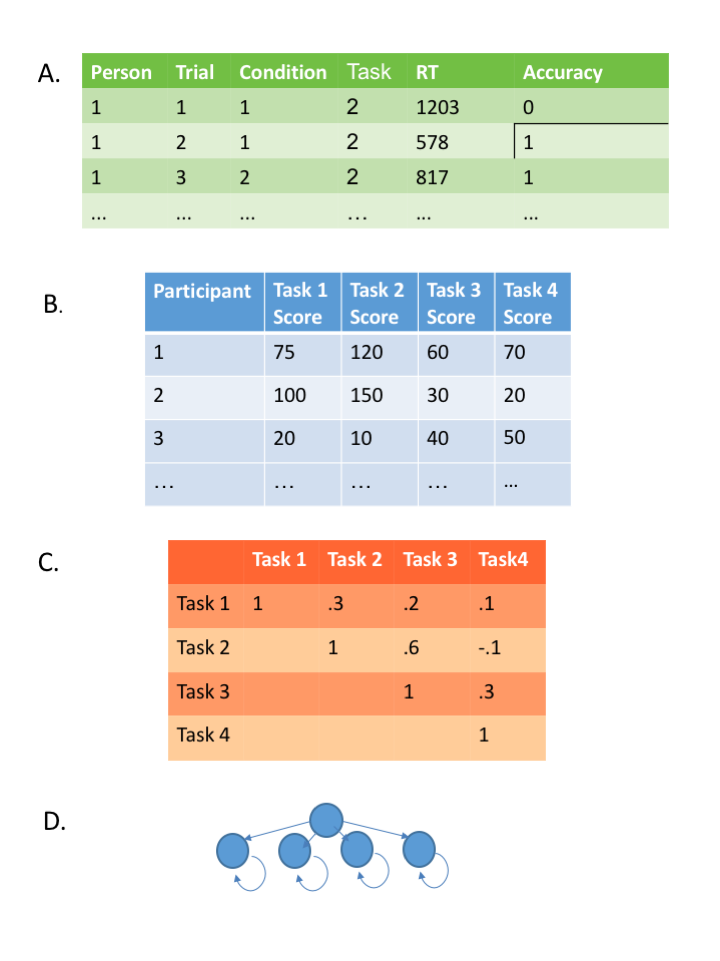
\includegraphics[width=4in]{dataAnalysis2} \caption{In the usual course of analysis, the raw data (A) are used to tabulate sample effects (B).  The covariation among these task-by-person sample effects (C) then serve as input to latent variable modeling (D).}\label{fig:usual}
\end{figure}

\begin{table}[tbp]

\begin{center}
\begin{threeparttable}

\caption{\label{tab:corTab}}

\begin{tabular}{llll}
\toprule
Study & Year & Correlation & Source\\
\midrule
Friedman \& Miyake & 2004 & 0.18 & Cited in Text\\
Unsworth \& Spillers & 2010 & 0.17 & Cited in Text\\
Unsworth \& McMillan & 2014 & 0.22 & Cited in Text\\
Shipstead et al. & 2014 & 0.11 & Cited in Text\\
Pettigrew \& Martin & 2014 & 0.03 & Cited in Text\\
Shipstead et al. & 2015 & 0.23 & Cited in Text\\
Redick et al. & 2015 & 0.17 & Cited in Text\\
Von Bastian et al. & 2016 & 0 & Computed\\
Hedge et al. & 2018 & -0.05 & Recomputed\\
Rey-Mermet et al. (ave) & 2018 & 0 & Recomputed\\
Whitehead et al. (ave) & 2019 & 0.03 & Recomputed\\
Draheim et al. & 2020 & 0.17 & Cited in Text\\
\bottomrule
\addlinespace
\end{tabular}

\begin{tablenotes}[para]
\normalsize{\textit{Note.} Recomputed correlations may differ from original source due to differences in cleaning steps.}
\end{tablenotes}

\end{threeparttable}
\end{center}

\end{table}

The above latent-variable approach to individual differences has been successful in some domains, such as personality, where rich factor structures are used to capture individual differences (Ashton et al., 2004; McCrae \& Costa Jr, 1997). Indeed, it seemed some twenty years ago that the same strategy would succeed in cognitive control (Kane \& Engle, 2003; Miyake et al., 2000). Yet, the latent-variable approach has not lived up to the promise, at least not in our opinion. Scores from experimental tasks correlate with one another far less than one might think \emph{a priori.} Take the correlation between Stroop and flanker tasks, two popular tasks for measuring inhibition. Table \ref{tab:corTab} shows some published values from the literature. As a rule, effects in inhibition tasks (as opposed to measures) show low correlations (Rey-Mermet, Gade, \& Oberauer, 2018). Indeed, even if we cherry pick the high end of these correlations, we tend not to find values about .3.

\begin{figure}
\centering
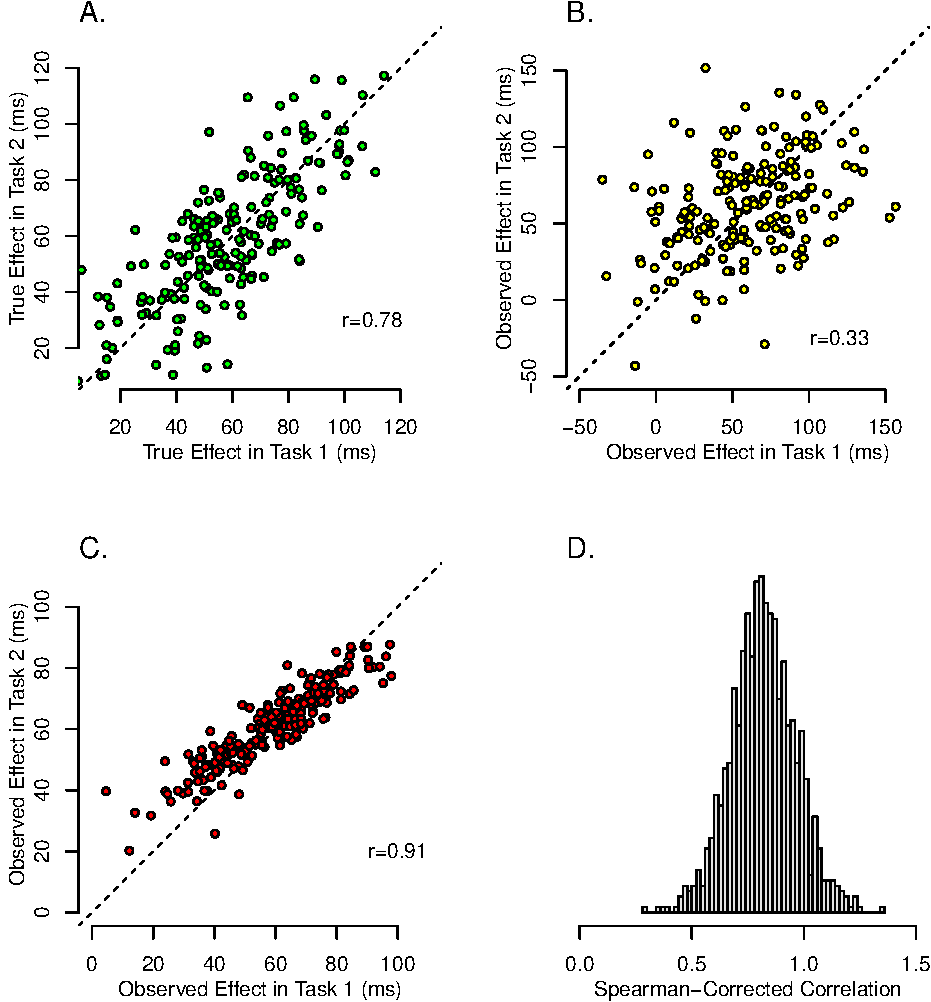
\includegraphics{p_files/figure-latex/example-1.pdf}
\caption{\label{fig:example}The effects of trial variability on the assessment of correlations among tasks. A: Hypothetical true individual effects show a large degree of correlation across two tasks. B: Observed effects are so perturbed by trial variability that the correlation is greatly attenuated. C: Hierarchical model recovery for the data in A. D: Spearman correction-for-attenuation in a small simulation with realistic settings.}
\end{figure}

The question of why these correlations are low has been the subject of recent work by Draheim, Mashburn, Martin, and Engle (2019), Hedge, Powell, and Sumner (2018) and Rey-Mermet, Gade, and Oberauer (2018) among others. On one hand, they could reflect underlying true task performance that is uncorrelated or weakly correlated. In this case, the low correlations indicate that performance on the tasks do not largely overlap, and that the tasks are indexing different mental processes. Indeed, this substantive interpretation is taken by Rey-Mermet, Gade, and Oberauer (2018), who argue that inhibition should be viewed as a disparate rather than a unified concept. By extension, different tasks rely on different and disparate inhibition processes.

On the other hand, the true correlations could be large but masked by measurement error. Several authors have noted the possibility of a large degree of measurement error. Hedge, Powell, and Sumner (2018), for example, set out to empirically assess the reliability of task measures by asking participants to perform a battery of tasks and to return three weeks later to repeat the battery. With these two measures, Hedge, Powell, and Sumner (2018) computed the test-retest reliability of the tasks. The results were somewhat disheartening with test-retest reliabilities for popular tasks in the range from .2 to .7. Draheim, Mashburn, Martin, and Engle (2019) argue that commonly used response time difference scores are susceptible to low reliability and other artifacts such as speed-accuracy tradeoffs.

It has been well known for over a century that correlations among measures are attenuated in low reliability environments (Spearman, 1904). Yet, how much attenuation can we expect? If it is negligible, then the observed low correlations may be interpreted as true indicators that the tasks are largely measuring uncorrelated mental abilities. But if the attenuation is sizable, then the underlying true correlation remains unknown. One of our contributions in this paper is to document just how big this attenuation is in common designs.

Figure \ref{fig:example} provides an example of attenuation. Shown in Panel A are hypothetical \emph{true difference scores} (or true effects) for 200 individuals on two tasks. The plot is a scatter plot---each point is for an individual; the x-axis value is the true score on one task, the y-axis value is the true score on the other task. As can be seen, there is a large correlation, in this case it is 0.78.
Researchers do not observe these true scores; instead they analyze difference scores from noisy trial data with the tabulation shown in Figure~\ref{fig:usual}. Figure \ref{fig:example}B shows the scatterplot of these observed difference scores (or observed effects). Because these observed effects reflect trial noise, the correlation is attenuated. In this case it is 0.33. While this correlation is statistically detectable, the observed value is dramatically lower than the true one.

The amount of attenuation of the correlation is dependent on critical inputs such as the number of trials and the degree of trial variability. Therefore, to get a realistic picture of the effects of measurement error it is critical to obtain realistic values for these inputs. In this paper, we survey 15 fairly large inhibition studies. From this survey, presented here subsequently, we derive typical values for the number of trials and the degree of trial variability. These typical values are used in Figure~\ref{fig:example}, and the amount of attenuation of the correlation therefore represents a typical rather than a worst-case scenario. As will be discussed, we believe that observed correlations in typical designs are less than 1/2 of the true values.

\hypertarget{measurement-error-and-trial-noise}{%
\section{Measurement Error and Trial Noise}\label{measurement-error-and-trial-noise}}

The amount of attenuation shown in Figure~\ref{fig:example}, from 0.78 to 0.33, is striking. No wonder it has been so hard to find correlations! What can be done? Our view is that there is a productive path by considering what contributes to measurement error (Rouder \& Haaf, 2019). Consider the workflow in Figure \ref{fig:usual} where the first analytic step is forming participant-by-task-score tables (Panel B). It is these scores that are susceptible to measurement error. But where does this error come from? The score is the differences in sample means, and the measurement error of these sample means is a function of the number of trials in the task. If there are a great many trials, then the sample means precisely estimate true means, sample differences precisely estimate true differences, and the correlation reflects the true correlation among the tasks. If there are few trials, then the sample means are variable and the observed correlation is attenuated. Hence, the number of trials per task is a critical quantity as it determines the systematic downward bias in correlation.

There are two immediate consequences to noting that the main component of measurement error is trial noise (Rouder \& Haaf, 2019). The first is that one cannot talk about the reliability of a task or the correlation among two tasks. These values are critically dependent on the number of trials. We cannot compare different values from different experiments without somehow accounting for differences in this design element. Simply put, there is no such thing as the reliability of a task or a correlation between tasks without reference to sample sizes. The second consequence is that the number of trials is far more important than the number of participants. The number of participants determines the unsystematic noise in the correlation; the number of trials determines the systematic downward bias. With few trials per task and many participants, researchers will have high confidence in a greatly biased estimate.

The realization that measurement error is primarily trial noise is wonderful news! It means that measurement error potentially may be overcome by running many trials per participant per condition per task. Even more importantly, trial noise can be estimated and perhaps removed using statistical techniques. The hope is that with such techniques, it may be possible to obtain unbiased estimates of the correlations even in realistic designs with limited numbers of trials per person per task. For example, Behseta, Berdyyeva, Olson, and Kass (2009), Haines et al. (2020), Matzke et al. (2017), Rouder and Haaf (2019), and Whitehead, Brewer, and Blais (2020) each propose hierarchical models to disattenuate correlations. The potential of such models is shown in Figure \ref{fig:example}C. Here, a hierarchical model, to be discussed subsequently, was applied to the data in \ref{fig:example}B, and the resulting posterior estimates of participants' effects reveal the true strong correlation.

Based on the demonstration in Figure \ref{fig:example}C, we had come into this research with the hope of telling a \emph{you-can-have-your-cake-and-eat-it} story. We thought that perhaps hierarchical models would allow for the accurate recovery of correlations in typical designs providing for an answer to whether cognitive control is unified or disparate. Yet, the story we tell here is far more complicated. First, we study 24 previously-published experiments to characterize the amount of measurement noise, true variability, and sample sizes in typical designs in inhibition-task research with individual differences. With these inputs, we then study correlation recovery through simulation. To foreshadow, overall estimates from hierarchical models do disattenuate correlations. But, in the course, they suffer from a large degree of imprecision. It seems that in typical designs, one can use sample statistics and suffer massive attenuation or use a modeling approach and accept a large degree of imprecision. And this difficulty is why we believe most studies of individual differences with tasks are doomed to fail. This story is not the one we had hoped to tell. It would have been much better for us if we could show that the models we advocate solve critical problems. But we cannot. And the inability to recover correlations even with the most sophisticated statistical approaches is an important story for the community of individual-differences scholars.

\hypertarget{spearmans-correction-for-attenuation}{%
\section{Spearman's Correction for Attenuation}\label{spearmans-correction-for-attenuation}}

Before addressing the main question about recovery, we consider the Spearman (1904) correction for the attenuation of correlation from measurement error. In this brief detour, we assess whether Spearman's correction leads to the recovery of latent correlations among tasks in typical designs. The assessment provides guidance because the data generation in simulations match well with the assumptions in Spearman's correction. If Spearman's correction cannot recover the latent correlations in realistic designs, these correlations may indeed be unrecoverable.

Spearman's derivation comes from decomposing observed variation into true variation and measurement noise. When reliabilities are low, correlations may be upweighted to account for them. In Spearman's classic formula, the disattenuated correlation, denoted \(r'_{xy}\) between two variables \(x\) and \(y\) is
\[
r'_{xy} = \frac{r_{xy}}{\sqrt{r_{xx}r_{yy}}},
\]
where \(r_{xy}\) is the sample correlation and \(r_{xx}\) and \(r_{yy}\) are the sample reliabilities.\footnote{The estimation of reliability in tasks is different than the estimation of reliability in a classical test because there are replicates within people and conditions in tasks. The presence of these replicates may be leveraged to produce better estimates of error variability than when they are not present. Let \(\bar{Y}_{ik}\) and \(s_{\bar{y}_{ik}}\) be the sample mean and sample standard error for the \(i\)th individual in the \(k\)th condition, \(k=1,2\). Let \(d_{i}=\bar{Y}_{i2}-\bar{Y}_{i1}\) be the effect for the \(i\)th individual, and let \(V_d\) be the sample variance of these effects. This sample variable is the total variance to be decomposed into true and error variances. Assuming an equal number of trials per condition, the error variance for the \(i\)th person, denoted \(V_{ei}\) is \(s^2_{\bar{y}_{i1}}+s^2_{\bar{y}_{i2}}\). The estimate of error variance is simply the average of these individual error variances, or \(V_e=\sum_i\sum_k s_{\bar{y}_{ik}}^2/I\). The reliability is \(r=(V_d-V_e)/V_d\).}

Spearman's correction, while well known, is not used often. The problem is that it is unstable. Panel D of Figure \ref{fig:example} shows the results of a small simulation based on realistic values from inhibition tasks discussed subsequently. The true correlation is .80. The Spearman-corrected correlations, however, are not only variable ranging from 0.38 to 1.72, but not restricted to valid ranges. In fact, 10.10\% of the simulated values are greater than 1.0. We should take these problems with Spearman's correction seriously. The poor results in Figure \ref{fig:example}D may indicate that in low-reliability environments, true correlations among tasks may not be recoverable. And this lack of recoverability may be fundamental---measurement noise may destroy the correlation signatures.

In this paper, we explore the recoverability of correlations in inhibition experimental tasks. We make our main claims by simulating data from known structures and then trying to recover signatures from experimental data. For these simulations to be useful, they must simulate data that have representative levels of true individual variation and of true trial noise. In the next section, we analyze existing data sets to find appropriate settings for simulations. With these settings established, we simulate data and assess whether correlations are recoverable. The hierarchical latent correlation estimators, while far from perfect, are better than Spearman-corrected correlation estimators. Subsequently, we apply the same analysis to a large data set from Rey-Mermet, Gade, and Oberauer (2018) spanning four inhibition tasks to assess whether the observed low correlations reflect independent task performance or attenuation from trial noise. Yet, even with hierarchical modeling, we are unable to definitively answer this question.

\hypertarget{variability-in-experimental-tasks}{%
\section{Variability in Experimental Tasks}\label{variability-in-experimental-tasks}}

To explore whether it is possible to recover correlations in typical designs, it is important to understand typical ranges of variability. Our approach is to gather a reasonable corpus of studies and analyze them, one-at-time, to understand the levels of true individual variation and trial noise. There are two issues: A. How to measure these levels of variation?, and B. Which extant studies to analyze? We take them in turn:

\hypertarget{one-task-measurement-model}{%
\subsection{One-Task Measurement Model}\label{one-task-measurement-model}}

To estimate within-trial and across-individual variabilities, we use an ordinary variance-components hierarchical model. To truly appreciate how variation can be assessed, the models need to be fully specified rather than left to short-hand. Let \(Y_{ijk\ell}\) be the \(\ell\)th response for the \(i\)th individual in the \(j\)th task and \(k\)th condition. In this section we analyze each task independently, so we may safely ignore \(j\), the task subscript (we will use it subsequently, however). The model for one task is:
\[
Y_{ik\ell} \sim \mbox{Normal}(\alpha_i+x_k\theta_i,\sigma^2),
\]
where \(\alpha_i\) is the \(i\)th individual's true response time in the congruent condition, \(x_k=0,1\) codes for the incongruent condition, \(\theta_i\) is the \(i\)th individual's true effect, and \(\sigma^2\) is the trial noise within an individual-by-condition cell. The critical target are the \(\theta_i\)s, and these are modeled as random effects:
\[
\theta_i \sim \mbox{Normal}(\mu_\theta,\sigma^2_\theta),
\]
where \(\mu_\theta\) describes the overall mean effect and \(\sigma^2_\theta\) is the between-person variation in individuals' true effects. Our targets then are the within-cell trial noise, \(\sigma^2\), and between-individual variance, \(\sigma^2_\theta\).

To analyze the model priors are needed for all parameters. Our strategy is to choose scientifically-informed priors (Dienes \& Mclatchie, 2018; Etz, Haaf, Rouder, \& Vandekerckhove, 2018; Rouder, Morey, \& Wagenmakers, 2016; Vanpaemel \& Lee, 2012) that anticipate the overall scale of the data. The parameters on baseline response times, in seconds, are \(\alpha_i \sim \mbox{Normal}(.8,1)\). These priors are quite broad and place no substantive constraints on the data other than baselines are somewhere around 800 ms plus or minus 2000 ms. The prior on variability is \(\sigma^2 \sim \mbox{Inverse Gamma}(.1,.1)\), where the inverse gamma is parameterized with shape and scale parameters (Rouder \& Lu, 2005). This prior, too, is broad and places no substantive constraint on data. Priors for \(\mu_\theta\) and \(\sigma^2_\theta\) were informed by the empirical observation that typical inhibition effects are in the range of 10 ms to 100 ms. They were \(\mu_\theta \sim \mbox{Normal}(50, 100^2 )\) and \(\sigma^2_\theta \sim \mbox{Inverse Gamma}(2,30^2)\), where the values are in milliseconds rather than seconds. A graph of these prior settings for \(\mu\) and \(\sigma_\theta=\sqrt{\sigma^2_\theta}\) is shown in Figure \ref{fig:theta}. These priors make the substantive assumption that effects are relatively small and are not arbitrarily variable across people. The scale setting on \(\sigma^2_\theta\) is important as it controls the amount of regularization in the model, and the choice of 30 (on the ms scale) is scientifically informed (see Haaf \& Rouder, 2017).

\begin{figure}
\centering
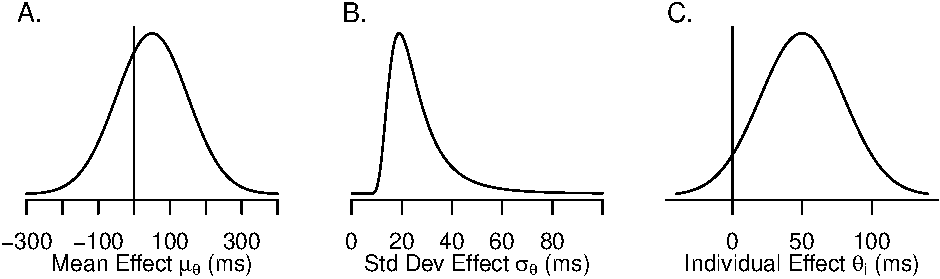
\includegraphics{p_files/figure-latex/theta-1.pdf}
\caption{\label{fig:theta}A, B: Prior distributions of \(\mu_\theta\) and \(\sigma_\theta\), respectively. C: Prior distribution of \(\theta_i\) for \(\mu_\theta=50\) ms and \(\sigma_\theta=30\) ms.}
\end{figure}

\begin{table}[tbp]

\begin{center}
\begin{threeparttable}

\caption{\label{tab:metaTab}}

\begin{tabular}{lllllllllll}
\toprule
 & \multicolumn{3}{c}{Sample Sizes} & \multicolumn{2}{c}{Reliability} & \multicolumn{2}{c}{Sample} & \multicolumn{2}{c}{Parameters} & \multicolumn{1}{c}{Ratio} \\
\cmidrule(r){2-4} \cmidrule(r){5-6} \cmidrule(r){7-8} \cmidrule(r){9-10} \cmidrule(r){11-11}
 & \multicolumn{1}{c}{Obs} & \multicolumn{1}{c}{Indv} & \multicolumn{1}{c}{Rep} & \multicolumn{1}{c}{Full} & \multicolumn{1}{c}{Split} & \multicolumn{1}{c}{Effect} & \multicolumn{1}{c}{$s_d$} & \multicolumn{1}{c}{$\hat{\sigma}$} & \multicolumn{1}{c}{$\hat{\sigma}_{\theta}$} & \multicolumn{1}{c}{$\hat{\eta}$}\\
\midrule
Stroop &  &  &  &  &  &  &  &  &  & \\
\ \ \ 1. von Bastian & 11,245 & 121 & 46 & 0.24 & 0.34 & 64 & 47 & 198 & 22 & 0.11\\
\ \ \ 2. Hedge & 43,408 & 53 & 410 & 0.83 & 0.75 & 69 & 32 & 188 & 29 & 0.16\\
\ \ \ 3. Pratte i & 11,114 & 38 & 146 & 0.61 & 0.68 & 91 & 50 & 264 & 36 & 0.14\\
\ \ \ 4. Pratte ii & 12,565 & 38 & 165 & 0.19 & -0.07 & 12 & 20 & 160 & 15 & 0.10\\
\ \ \ 5. Rey-Mermet i & 48,937 & 264 & 93 & 0.40 & 0.57 & 54 & 30 & 155 & 18 & 0.12\\
\ \ \ 6. Rey-Mermet ii & 48,966 & 261 & 94 & 0.86 & 0.84 & 59 & 69 & 174 & 64 & 0.36\\
\ \ \ 7. Whitehead i & 122,547 & 178 & 344 & 0.70 & 0.71 & 76 & 53 & 378 & 44 & 0.12\\
\ \ \ 8. Whitehead ii & 133,966 & 194 & 345 & 0.56 & 0.63 & 78 & 52 & 408 & 37 & 0.09\\
\ \ \ 9. Whitehead iii & 125,979 & 210 & 300 & 0.57 & 0.51 & 116 & 50 & 402 & 37 & 0.09\\
Simon &  &  &  &  &  &  &  &  &  & \\
\ \ \ 10. von Bastian & 23,453 & 121 & 97 & 0.60 & 0.61 & 79 & 36 & 128 & 28 & 0.22\\
\ \ \ 11. Pratte i & 17,343 & 38 & 228 & 0.46 & 0.62 & 17 & 24 & 186 & 18 & 0.10\\
\ \ \ 12. Pratte ii & 12,266 & 38 & 161 & 0.57 & 0.51 & 30 & 30 & 175 & 23 & 0.13\\
\ \ \ 13. Whitehead i & 127,036 & 178 & 357 & 0.71 & 0.72 & 67 & 29 & 205 & 24 & 0.12\\
\ \ \ 14. Whitehead ii & 139,332 & 194 & 359 & 0.56 & 0.59 & 66 & 26 & 212 & 19 & 0.09\\
\ \ \ 15. Whitehead iii & 125,953 & 210 & 300 & 0.66 & 0.66 & 102 & 28 & 201 & 23 & 0.11\\
Flanker &  &  &  &  &  &  &  &  &  & \\
\ \ \ 16. von Bastian & 11,215 & 121 & 46 & -0.02 & -0.55 & 2 & 32 & 152 & 15 & 0.10\\
\ \ \ 17. Hedge & 43,384 & 53 & 409 & 0.80 & 0.79 & 44 & 16 & 100 & 15 & 0.15\\
\ \ \ 18. Rey-Mermet i & 49,300 & 265 & 93 & 0.18 & 0.17 & 30 & 24 & 147 & 13 & 0.09\\
\ \ \ 19. Rey-Mermet ii & 39,275 & 207 & 95 & 0.87 & 0.87 & 36 & 43 & 107 & 40 & 0.37\\
\ \ \ 20. Whitehead i & 126,987 & 178 & 357 & 0.62 & 0.61 & 47 & 33 & 265 & 25 & 0.10\\
\ \ \ 21. Whitehead ii & 139,103 & 194 & 359 & 0.19 & 0.19 & 32 & 26 & 272 & 14 & 0.05\\
\ \ \ 22. Whitehead iii & 125,918 & 210 & 300 & 0.38 & 0.41 & 61 & 30 & 290 & 19 & 0.07\\
Other &  &  &  &  &  &  &  &  &  & \\
\ \ \ 23. Rouder i & 11,346 & 52 & 109 & 0.37 & 0.35 & 50 & 28 & 165 & 19 & 0.11\\
\ \ \ 24. Rouder ii & 16,859 & 58 & 145 & 0.62 & 0.62 & 142 & 72 & 351 & 53 & 0.15\\ \midrule
Mean & 65,312 & 145 & 223 & 0.52 & 0.51 & 59 & 37 & 220 & 27 & 0.14\\
Median & 46,172 & 178 & 197 & 0.57 & 0.61 & 60 & 31 & 193 & 23 & 0.11\\
\bottomrule
\addlinespace
\end{tabular}

\begin{tablenotes}[para]
\normalsize{\textit{Note.} All sample sizes and estimates reflect cleaned data.  See the Appendix for our cleaning steps which differ from those of the original authors.}
\end{tablenotes}

\end{threeparttable}
\end{center}

\end{table}

\hypertarget{data-sets}{%
\subsection{Data Sets}\label{data-sets}}

We applied this model to a collection of 24 experimental tasks from a variety of authors. Brief descriptions of the tasks are provided in the Appendix. It is reasonable to ask why these 24 and whether they are representative.
The experiments were chosen based on the following three criteria: I. Raw trial-level data were available and adequately documented. This criterion is necessary because model analysis relies on the raw data and cannot be performed with the usual summary statistics. II. These raw data could be shared. This research is offered within a fully open and transparent mode (Rouder, Haaf, \& Snyder, 2019), and you may inspect all steps from raw data to conclusions. III. The data come from an experimental setup where there was a contrast between conditions; i.e., between congruent and incongruent conditions.

Are these studies representative? Representativeness is assessed relative to the goals of the analysis. The goals here are to ascertain representative values of trial variation (\(\sigma^2\)) and the true variability in the population after accounting for trial noise (\(\sigma^2_\theta\)). Representativeness is not about whether these data sets show high or low correlations among tasks as tasks are analyzed independently and correlations are orthogonal to the variabilities of interest. Representativeness is not about power or number of participants. All the studies we considered are well powered for estimating the variabilities, and it is the variabilities that are key. So, it is fair to ask if these studies are representative for estimating variabilities. We return to this question after describing the results.

The results from applying the one-task measurement model to the 24 sets are shown in Table \ref{tab:metaTab}. The first three columns describe the sample sizes: The first column is the total number of observations across the two conditions after cleaning (see Appendix), the second column is the total number of individuals, and the third column is the average number of replicates per individual per condition. The fourth and fifth columns provide estimates of reliability. The column labeled ``Full'' is the sample reliability using all the observations in one group (see Footnote 1); the column labeled ``Split'' is the split-half reliability. Here, even and odd trials comprised two groups and the correlation of individuals' effects across these groups was upweighted by the Spearman-Brown prophecy formula. Note that the former estimate is more accurate than the split-half estimate because the former uses variability information across trials, much like in ANOVA, where the later does not. The next pair of columns shows the mean sample effect and the standard deviation of individuals' sample effects around this mean. These are sample statistics calculated in the usual way and do not reflect the model. The next two columns are standard deviation estimates from the hierarchical model. The column \(\hat{\sigma}\) is the posterior mean for residual variability and the column \(\hat{\sigma}_\theta\) is the posterior mean for the true variability across individuals. The final column, labeled \(\hat{\eta}\), is the ratio of these standard deviations. As discussed subsequently, this ratio reflects how reliable the task is and how much the naive correlations will be attenuated.

In hierarchical models, the estimate of true variability across people, \(\sigma_\theta\) is smaller than the variability among sample effects (\(s_d\) in the table). The reason is straightforward---\(s_d\) contains contributions from both individual variability and trial noise. The phenomenon is sometimes called \emph{hierarchical shrinkage} or \emph{hierarchical regularization}, and a brilliant explanation is provided in Efron and Morris (1977). Rouder and Haaf (2019) extend this explanation to inhibition tasks, and the reader is referred to these sources for further discussion.

We don't know if these 24 studies are representative of a larger corpus simply because researchers do not often model trial noise separate from true individual variability. In some sense, we are the first here, and the analysis of these 24 is the most comprehensive testbed for this question to date. We are sanguine that we have covered a broad range of possibilities. Take, for example, the large range covered by the Hedge et al.~flanker study which is characterized by a small degree of trial noise (\(\sigma=100\) ms) on one hand, and the Whitehead et al.~Stroop studies, which are characterized by a large degree of trial noise (\(\sigma \approx 400\) ms) on the other. Likewise, some studies have a low degree of true individual variation while others have a larger degree. The good news is that although the studies vary, all the values stay in the same order of magnitude, and there is much stability in the ratio of true individual variation and trial noise. We think the analyses of these 24 is novel, highly informative, and forms the new state-of-the art for expectations about these variabilities.

From the table, we derive the following critical values for the following simulations. We set the trial-by-trial variation to \(\sigma= 200\) ms, and the variation of individuals' true effects to \(\sigma_\theta=25\) ms. The critical choice is the latter, and a reader may question its small size. Does it make sense, and why is the larger value \(s_d\), the empirically observed standard deviation of individuals effect scores not used. The values \(s_d\) are larger because they necessarily include contributions from trial noise and variability across individuals. The second column, \(s_\theta\) reflects the model's partition of variance, that is, what is left over after trial noise, given by \(\sigma\), is accounted for. Given the assumptions of the model, it reflects only the variability across individuals. Hence, it is the far better value for simulation.

We provide a second argument that may be more intuitive for understanding the 25 ms value. Consider the possibility that all people truly respond faster in the congruent than in the incongruent condition. Or, restated, nobody has a negative true effect. Again, we emphasize the difference between true effects and observed effects. Obviously even when all people truly respond faster in the congruent condition, some people will have observed effects in the opposite direction simply from trial noise. How would one know if all true effects are in the same direction. We developed Bayes factor solutions for just this question (Haaf \& Rouder, 2017, 2019; Rouder \& Haaf, 2021). When every participant shows a true effect in the same direction, we say dominance is observed (Rouder \& Haaf, 2018). The best evidence to date is that dominance holds in priming and conflict tasks (Rouder \& Haaf, 2021). In the Stroop case, we are sure that everyone Stroops, that is, in the large trial limit, everyone has truly faster scores for congruent than incongruent stimuli (Haaf \& Rouder, 2017).

If dominance holds and the true mean effect is small across the population, say 50 ms, then the variance between individuals cannot be too high. For if it were large, then some proportion of people must have negative true effects. Dominance---which is natural and seems to hold in almost all sets we have examined---provides a limit on the size of variability. Figure \ref{fig:theta} provides a graph of true values with a spread of 25 ms. As can be seen, there is only minimal mass for negative true values, and the spread of true values to us seems appropriate for a true 50 ms effect.

\hypertarget{expected-attenuation}{%
\section{Expected Attenuation}\label{expected-attenuation}}

The above results are useful for understanding how much attenuation of the correlations we should expect with the usual analysis in Figure \ref{fig:usual}. We consider the case where in each task there are \(L\) trials per task per condition, common trial variance \(\sigma^2\) and common true variance \(\sigma^2_\theta\). The expected classical estimate, \(\rho^*\), is given by
\[
\rho^* = \rho\left(\frac{L\sigma^2_\theta}{L\sigma^2_\theta+2\sigma^2}\right).
\]
This equation is most useful if written with the ratio \(\eta=\sqrt{\sigma_\theta/ \sigma}\), with this ratio interpreted as a ratio of signal (true variability) to noise (trial noise). Then, the attenuation factor, \(\rho^*/\rho\) is
\begin{equation} \label{eq:fid}
\frac{\rho^*}{\rho} = \left( \frac{L}{L+2/\eta^2}\right).
\end{equation}
{]}
The last column of Table \ref{tab:metaTab} shows the value of \(\eta\) for the various studies, and the values range from 1/11 to 1/3, with \(\eta=1/8\) corresponding to our typical case. Figure \ref{fig:attenuate} shows the dependence of the attenuation factor on the number of trials (\(L\)) for various values of signal to noise. As can be seen, with the usual approach of tabulating participant-by-task scores, we expect attenuation to be a factor of .44 for \(L=100\) replicates.

\begin{figure}
\centering
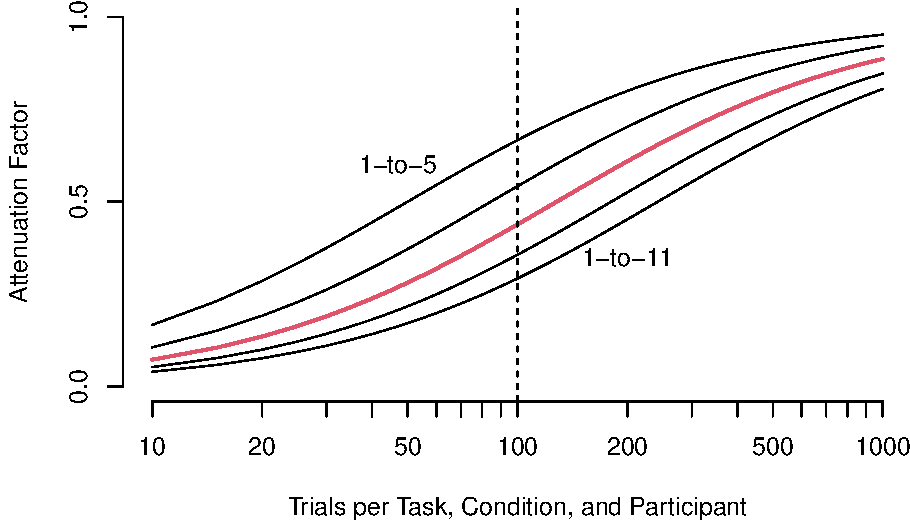
\includegraphics{p_files/figure-latex/attenuate-1.pdf}
\caption{\label{fig:attenuate}Attenuation of correlation as a function of number of trials (\(L\)) and signal-to-noise ratio \(\eta\). For typical values (\(L=100\), \(\eta\)=1-to-8), the attenuation is a factor of 44. The plotted values of \(\eta\) are 1-to-5, 1-to-6.5, 1-to-8, 1-to-9.5, and 1-to-11.}
\end{figure}

\hypertarget{model-based-recovery-of-correlations-among-tasks}{%
\section{Model-Based Recovery of Correlations Among Tasks}\label{model-based-recovery-of-correlations-among-tasks}}

The critical question is then whether accurate estimation of correlation is possible. The small simulation in the introduction, which was based on the above typical settings for two tasks and a true population correlation of .80, showed that naive correlations among sample effects were greatly attenuated and Spearman's correction was unstable. We now assess the recoverability of true latent correlations with the hierarchical models used to simulate data and for several values of true correlations.

\hypertarget{a-hierarchical-model-for-correlation}{%
\subsection{A Hierarchical Model for Correlation}\label{a-hierarchical-model-for-correlation}}

Here we develop a hierarchical trial-level model for many tasks that explicitly models the covariation in performance among them. A precursor to this model is provided in Matzke et al. (2017) and Rouder and Haaf (2019). A similar mixed-linear model is provides in Whitehead, Brewer, and Blais (2020). The difference is that these previous models are applicable for only two tasks and one correlation coefficient. They are not applicable to several tasks and coefficients.

At the top level, the model is:
\[
Y_{ijk\ell} \sim \mbox{Normal}(\alpha_{ij}+x_k\theta_{ij},\sigma^2).
\]
The target of inquiry is \(\theta_{ij}\) the effect for the \(i\)th participant in the \(j\)th task. The specification is made easier with a bit of vector and matrix notation. Let \(\bftheta_{i}=(\theta_{i1},\ldots,\theta_{iJ})'\) be a column vector of the \(i\)th individual's true effects. This vector comes from a group-level multivariate distribution. The following is the case for three tasks:

\[
\bftheta_i=\begin{bmatrix} \theta_{i1}\\ \theta_{i2} \\ \theta_{i3}\end{bmatrix} 
\sim \mbox{N}_3 \left( \begin{bmatrix} \mu_1\\\mu_2\\\mu_3\end{bmatrix},
\begin{bmatrix}
\sigma^2_{\theta_1} & \rho_{12}\sigma_{\theta_1}\sigma_{\theta_2} & \rho_{13}\sigma_{\theta_1}\sigma_{\theta_3}\\
\rho_{12}\sigma_{\theta_1}\sigma_{\theta_2} & \sigma_{\theta_2}^2 & \rho_{23}\sigma_{\theta_2}\sigma_{\theta_3}\\
\rho_{13}\sigma_{\theta_1}\sigma_{\theta_3} & \rho_{23}\sigma_{\theta_2}\sigma_{\theta_3} & \sigma_{\theta_3}^2\\
\end{bmatrix}
\right).
\]
More generally, for \(J\) tasks,
\begin{equation}
\label{eq:Sig}
\bftheta_i \sim \mbox{N}_J(\bfmu,\bfSigma_\theta).
\end{equation}

Priors are needed for \(\bfmu\), the vector of task means, and \(\bfSigma_\theta\), the covariance across the tasks. We take the same strategy of using scientifically-informed priors. For \(\bfmu\), we place the normal in Figure~\ref{fig:theta}A on each element. For \(\bfSigma_\theta\), the classic choice is the \emph{inverse Wishart} prior. This choice is popular because it is flexible and computationally convenient (O'Hagan \& Forster, 2004). The inverse Wishart requires a scale parameter, and we set it so that the marginal prior on standard deviations of true variation matches the distribution in \ref{fig:theta}B.\footnote{There is an alternative choice of prior for covariance that we extensively explored, the \emph{LKJ prior} (Lewandowski, Kurowicka, \& Joe, 2009). This prior is less informative than the Wishart because, unlike the Wishart, the estimation of correlation is independent of the specification of scale. Consequently, this prior is recommended (McElreath, 2016), and implementation is convenient in the \texttt{R}-package \texttt{rstan} (Stan Development Team, 2018). Yet, we found better performance for the inverse Wishart in simulations in that the posterior credible intervals were smaller and better covered the true value. The increased performance of the Wishart reflects the fact that researchers have a rough idea about the scale of individual differences---it is on the order of tens of milliseconds---and this is enough information for the improved performance of the inverse Wishart.} It is the use of the inverse Wishart here that allows the model to be applicable to many tasks and correlation coefficients.

\hypertarget{two-tasks}{%
\subsection{Two Tasks}\label{two-tasks}}

The first simulation is for two tasks. In performing simulations, we must set the sample sizes, ground truth relations among the tasks, trial noise and true individual variation. The former two were set by the preceding analysis. For all of our simulations, we used \(I=200\) people and \(L=100\) replicates per condition. We think these are good choices to emulate designs where many individuals are going to run in several inhibition tasks. For tasks with two conditions, there are 40,000 observations per task. In a typical battery with \(J=10\) tasks, the total number of observations is 400,000, which is quite large. Hence, our choices seem appropriate to typical large-scale individual-difference studies with experimental tasks.

Using the typical sample sizes discussed above, each hypothetical data set consisted of 80,000 observations (200 people \(\times\) 2 tasks \(\times\) 2 conditions \(\times\) 100 replicates per condition). One might hope that with such a large sample size and with a goal of estimating a single correlation, the true population correlation, \(\rho\), might be recoverable. Supporting this hope is the success of the single run in Figure \ref{fig:attenuate}C. On the other hand, given the large degree of measurement noise and the instability of Spearman's correction (Figure \ref{fig:attenuate}B), it seems plausible that \(\rho\) may not be recoverable.

The last input to the simulations are the ground true correlations. We have the possibility of exploring recovery across a wide range of possible relationships among tasks. For the simulations, true correlation values across the two tasks were varied on three levels with values of .2, .5, and .8, representing tasks with low, high, and very high levels of correlation. For each of these levels, 100 data sets were simulated and analyzed.

\begin{figure}
\centering
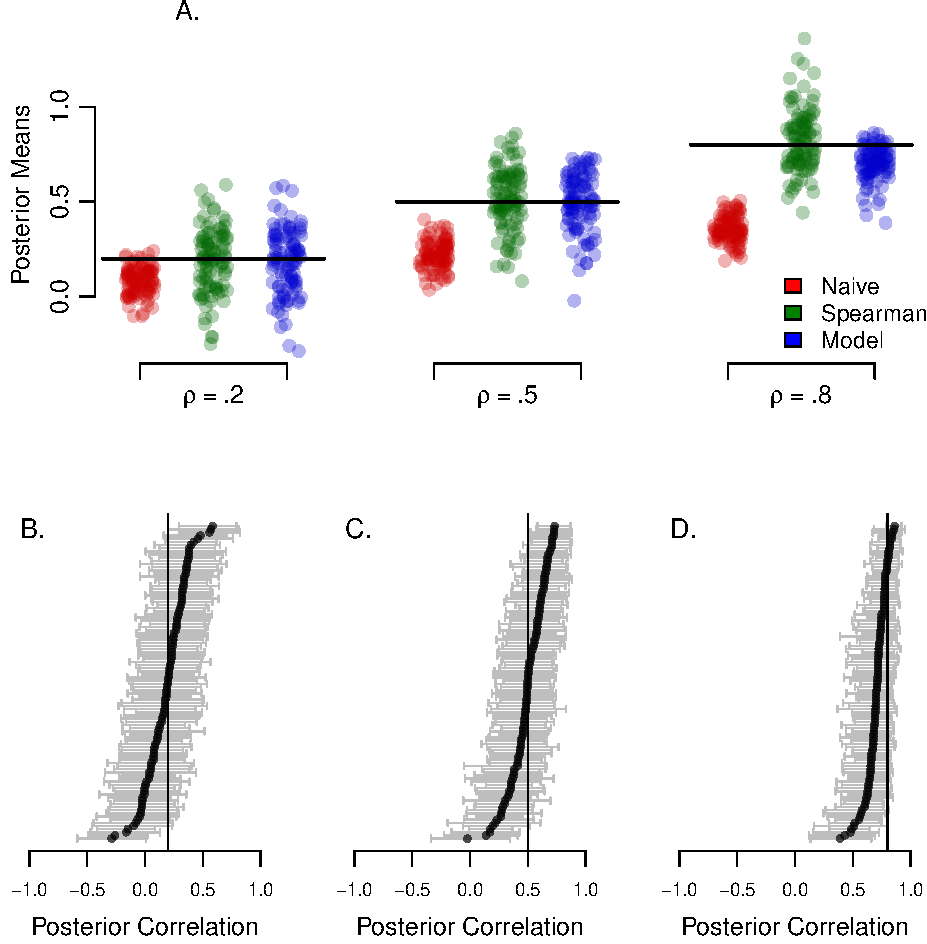
\includegraphics{p_files/figure-latex/recov2-1.pdf}
\caption{\label{fig:recov2}Revocery of correlations from two tasks. A: Boxplots of recovered correlations from naive sample correlations, Spearman's correction, and the hierarchical model. B-D: Posterior 95\% credible intervals for the model-recovered correlations for true correlations of .2, .5, and .8, respectively.}
\end{figure}

Figure \ref{fig:recov2}A shows the results. Naive correlations from participant-by-task sample means are shown in red. As expected, these correlations suffer a large degree of attenuation from trial noise. Correlation estimates from Spearman's correction are shown in green. These values are better centered though some of the corrected values are greater than 1.0. The correlation estimates from the hierarchical model are shown in blue.

Overall, the correlation estimates from Spearman's correction and the hierarchical model have less bias than the naive sample-effect correlations. Yet, the estimates are quite variable. For example, consider correlations when the population value is .2. The model estimates range from -0.29 to 0.58 and miss the target with a RMSE of 0.17. Spearman corrected estimates are a slightly better and have an RMSE for this case of 0.17. Overall though, this variability is quite high especially given the large number of observations. We would not have confidence in substantive conclusions with it.

Are there risks in using model-based recovery? We see in simulation that the model and Spearman-corrected recovery is variable. One potential problem is that in any one study, researchers using the model inflate the values of correlations. The attenuation in the naive correlations is conservative in that recovered correlations are never inflated, rather, they are dramatically deflated. In this regard, we can think of naive-correlations as having a fail-safe quality where high-value correlation estimates are avoided at the draconian expense of not detecting true high correlations. Spearman-corrected correlations do not share this fail-safe orientation. The variability in estimation results in values that are both inflated and deflated.

The critical question is about model-based recovery. Figure \ref{fig:recov2}A shows only posterior mean estimates. Yet, in the Bayesian approach, the target is not just the posterior mean, but the entirety of the posterior distribution. Figure \ref{fig:recov2}B-D shows the posterior 95\% credible intervals for all runs with true correlations of .2, .5, and .8, respectively. There are two noteworthy trends. First, the 95\% credible intervals tend to contain the true value on 89\% of the simulation runs. This means that the posterior variability is relatively well calibrated and provides reasonably accurate information on the uncertainty in the correlation. Second, there is a fair amount of uncertainty meaning that the analyst knows that correlations have not been well localized. This lack of localization provides the needed hedge for over interpreting inflated values. With the Bayesian model-based estimates, at least we know how uncertain we are in localizing true correlations. With the Spearman correction, we have no such knowledge.

\hypertarget{six-tasks}{%
\subsection{Six Tasks}\label{six-tasks}}

We explored correlations across six tasks. Each hypothetical data set consisted of 240,000 observations. To generate a wide range of correlations, we used a one-factor model to simulate individuals' true scores. This factor represents the individual's inhibition ability. This ability, denoted \(z_i\), is distributed as a standard normal. Tasks may require more or less of the individuals' inhibition ability. Therefore, task loadings onto this factor \(z_i\) are variable and, as a result, a wide range of correlations occur. The following task loading values work well in producing a diversity of correlations: 1.5 ms, 5.7 ms, 9.9 ms, 14.1 ms, 18.3 ms, and 22.5 ms. Following the one-factor structure we may generate true scores, \(\theta_{ij}\), for each task and participant:
\[
\theta_{ij} \sim \mbox{Normal}(\mu_j+z_iw_j,\eta^2),
\]
where \(z_i\) is the true ability, \(w_j\) is the task loading, \(\mu_j\) is the task overall mean, and \(\eta^2\) is residual variability in addition to that from the factors. In simulation we set \(\eta=10\) ms, and this setting yields standard deviations across \(\theta_{ij}\) between 10 ms and 30 ms, which is similar to the 25 ms value used previously. The true population variance for the one-factor model is \(\bfSigma = \bfw\bfw' + \bfI\eta^2\), where \(\bfw\bfw'\) is the matrix formed by the outer product of the task loadings. The true correlation matrix from the variance-covariance matrix \(\bfSigma\) is shown in Figure \ref{fig:cov6}A, and the values subtend a large range from near zero to 0.80.

\begin{figure}
\centering
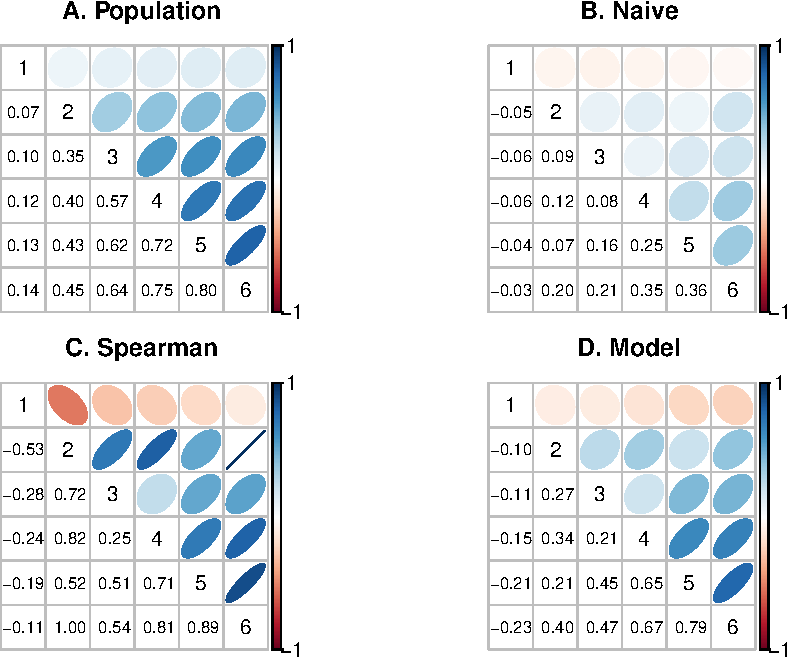
\includegraphics{p_files/figure-latex/cov6-1.pdf}
\caption{\label{fig:cov6}True and recovered correlation matrices for six tasks. A: True population correlations. B-D: Correlation estimates from a single run.}
\end{figure}

\begin{figure}
\centering
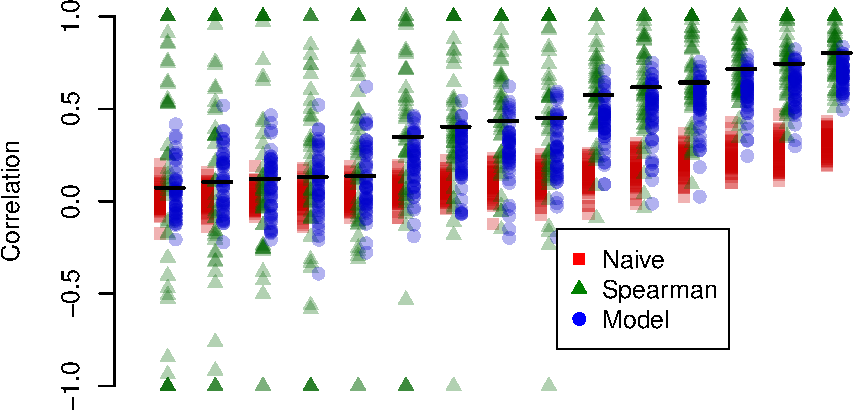
\includegraphics{p_files/figure-latex/recov6-1.pdf}
\caption{\label{fig:recov6}Recovery of correlations from six tasks. True correlations are derived from a one-factor model and are displayed in Figure \ref{fig:cov6}.}
\end{figure}

The recovery of correlations is shown for a single simulation run in Figure \ref{fig:cov6}B-D. The attenuation for the naive correlations is evident, as is variability in model-based and Spearman corrected estimates. Figure \ref{fig:recov6} shows the performance of the methods across the 50 simulation runs.\\
As can be seen, there remains the dramatic attenuation for the naive correlation of sample effects and excessive variability for the Spearman-corrected and model-based correlation estimates. Spearman corrected estimates are free to be outside the valid range from -1 to 1. We imagine that any researcher encountering these values could justifiably set them to the appropriate endpoint, and we do so in Figure \ref{fig:recov6}. Nonetheless, the RMS errors remain high---across the whole range of true values they are 0.59 and 0.19 for the Spearman correlation and model, respectively. It is somewhat heartening that model recovery is somewhat informative.

\hypertarget{analysis-of-rey-mermet-gade-and-oberauer-2018}{%
\section{Analysis of Rey-Mermet, Gade, and Oberauer (2018)}\label{analysis-of-rey-mermet-gade-and-oberauer-2018}}

To assess real-world correlation recovery, we re-examined the flanker and Stroop tasks in Rey-Mermet et al.'s battery of inhibition tasks. The authors included two different types of Stroop tasks (a number Stroop and a color Stroop task, see the Appendix for details) and two different types of flanker tasks (a letter flanker and an arrow flanker task, see the Appendix for details). The question then is about the correlation across the tasks.\footnote{One of the elements that makes analysis complicated is how to exclude low-performing participants. In the previous analysis, where each task was analyzed in isolation, we retained all participants in a task who performed over 90\% accuracy on that task. In the current analysis, however, we must have the same participants for all four tasks. We decided to retain those participants who have over 90\% accuracy on all four tasks. With this strict criterion, we retain only 180 of the original 289 participants. The most noticeable effect of this exclusion is that the reliability for the arrow flanker task was reduced from .87 to .56. The fact that the reliability changes so much indicates that the high reliability was driven by a few participants with very large difference scores. This cutoff differs from Rey-Mermet, Gade, and Oberauer (2018), who used a 75\% accuracy. With this lower cutoff, they included many more participants.}

\begin{figure}
\centering
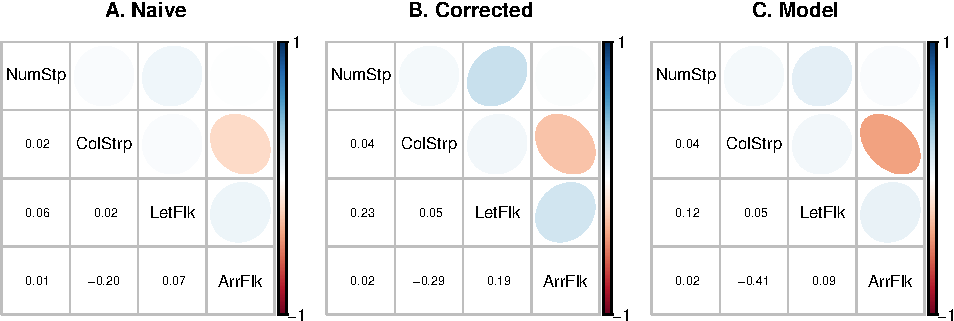
\includegraphics{p_files/figure-latex/rm4task-1.pdf}
\caption{\label{fig:rm4task}Correlations among select tasks in the Rey-Mermet data set. Tasks are a number Stroop task, a color Stroop task, a letter flanker task, and an arrow flanker task. Details of the tasks are provided in the Appendix.}
\end{figure}

\begin{figure}
\centering
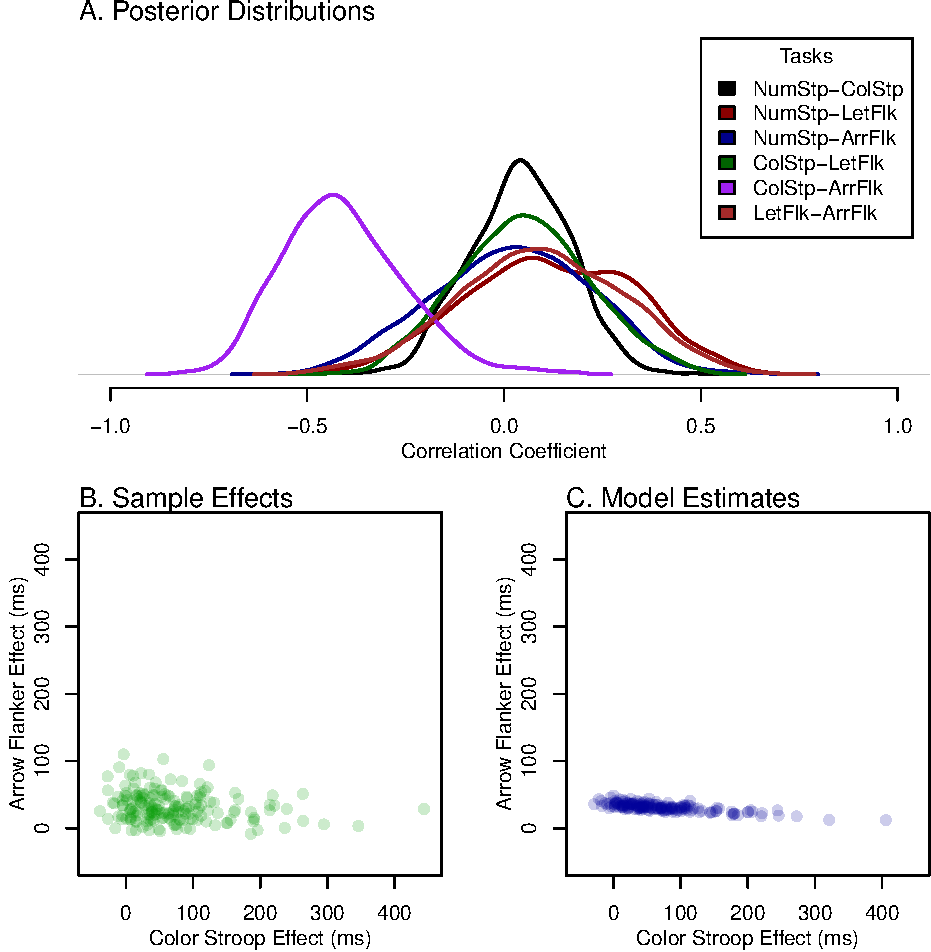
\includegraphics{p_files/figure-latex/rm4taskEst-1.pdf}
\caption{\label{fig:rm4taskEst}A. Model-based posterior distributions of population correlations among tasks. The large variance shows the difficulty of recovery. B. Individuals' sample effects for color Stroop and arrow flanker tasks show. C. Hierarchical model estimates show a large degree of shrinakge for arrow flankers but not for color Stroop reflecting the increased range of color Stroop effects.}
\end{figure}

The top three rows of Figure \ref{fig:rm4task} show the estimated correlations from sample effects, Spearman's correction, and the hierarchical model. Given the previous simulations results, it is hard to know how much credence to give these estimated correlations. In particular, it is hard to know how to interpret the negative correlation between the arrow flanker and color Stroop task.

To better understand what may be concluded about the range of correlations, we plot the posterior distribution of the correlation (Figure \ref{fig:rm4taskEst}A). These distributions are unsettling. The variation in most of these posteriors is so wide that firm conclusions are not possible. The exception is the null correlation between number and color Stroop which seems to be somewhat well localized. The surprisingly negative correlation between color Stroop and arrow flanker comes from a posterior so broad that the 95\% credible interval is {[}-0.27,0.39{]}. Here, all we can say is that very extreme correlations are not feasible. We suspect this limited result is not news.

Analysis of Rey-Mermet, Gade, and Oberauer (2018) provides an opportunity to examine how hierarchical models account for variation across trials as well as variation across people. Figure \ref{fig:rm4taskEst}B shows sample effects across individuals for the color Stroop and arrow flanker tasks, the two tasks that were most negatively correlated. There is a far greater degree of variation in individual's effects for the color Stroop task than for the arrow flanker task. The model estimates (Figure \ref{fig:rm4taskEst}C) reflect this difference in variation. The variation in arrow flanker is so small that it can be accounted for with trial variation alone. As a result, the hierarchical model shows almost no individual variability. In contrast, the variability in the color Stroop is large and the main contributor is true variation across individuals rather than trial variation. Hence, there is relatively little shrinkage in model estimates. The lack of variation in the arrow flanker task gives rise to the uncertainty in the recovered correlation between the two tasks.

\hypertarget{general-discussion}{%
\section{General Discussion}\label{general-discussion}}

A basic question facing researchers in cognitive control is whether inhibition is a unified phenomenon or a disparate set of phenomena. A natural way of addressing this question is to study the pattern of individual differences across several inhibition tasks. In this paper, we have explored whether correlations across inhibition tasks may be recovered. We consider typically large studies that enroll hundreds of participants and run tasks with 100s of usable trials per condition. The answer is largely negative---correlations are difficult to recover with accuracy that would allow for a definitive answer to this basic question. This statement of poor recovery holds for hierarchical models that are extended to the trial level.

Why this depressing state-of-affairs occurs is fairly straightforward. Relative to trial noise, there is little true individual variation in inhibition tasks. To see why this is so, consider an average effect, say one that is 60 ms. In inhibition tasks like Stroop and flanker, we can safely make a \emph{dominance assumption}---nobody truly has a negative effect (Haaf \& Rouder, 2017). That is to say nobody truly identifies incongruent stimuli faster than congruent ones. Under this assumption, where all true scores are positive, a small mean necessarily implies a small variance. For example, if true Stroop effects are reasonably normally shaped, the mean is 60 ms and there can be no mass below zero, then an upper bound on variability across true scores is a standard deviation of 25 ms or so. This is a small amount of variation compared to trial variability, which is typically 8 times larger. This small degree of true variation necessarily implies a small degree of covariation across tasks. And this small degree of covariation is beyond the resolution of our experimental designs, and that is why our data are difficult.

We believe this problem of localizing individual differences and correlations extends beyond inhibition tasks. It likely holds broadly in most task domains as most tasks have relatively small effects, whether on the order of 60 ms for RT, on the order of .08 for accuracy, or maybe on the order of 1/10th of the scale for Likert values. If we make a dominance assumption---each individual has a true effect in the same direction---then there cannot be much individual variability else these mean effects would be larger. And measuring correlations with small degrees of individual variability may be beyond the resolution of typical designs.

\hypertarget{recommendations}{%
\subsection{Recommendations}\label{recommendations}}

Based on the above correlation-recovery results, we can make the following recommendations:

\emph{Be mindful of attenuation}. Researchers have certainly been aware of measurement error and understand the link between measurement error and attenuation. Yet, in our view, they have not asked the tough questions. Can correlations be estimated in low and medium reliability environments? Can the factor structures be accurately recovered in low-reliability environments? How difficult is it to conclude that there is a lack or a small correlation in such environments? Previous to this work, there were no systematic studies of the degree of attenuation, and hence little basis to understand its effects. Here, we argue that the critical factor---the ratio of true variability to trial noise---is on the order of 1-to-8, and may be as great as 1-to-11. Now, for various numbers of trials, researchers can compute how much attenuation is expected using Equation (\ref{eq:fid}). These values can be used for sample size planning and as context in interpretation.

\emph{Stress the number of trials in a task}. Typically, researchers are quick to report the number of participants they have run. These numbers appear not only in method sections, but in abstracts and tables. And researchers may believe that with larger numbers of participants, results are better powered and become more accurate. This belief is wrong, especially in low reliability environments. The more critical design element is the number of trials per person within a task. With few trials, there is much trial noise and much attenuation. Low numbers of trials add systematic bias whereas low numbers of people add unsystematic noise. Moreover, using high numbers of participants with low numbers of trials breeds high confidence in a wrong answer. We recommend researchers consider running fewer tasks and conditions to gain larger numbers of trials per task. Moreover, we recommend researchers stress the role of the number of trials in their discussion and report these numbers in their method sections, tables, and abstracts.

\emph{Stop Aggregating Trial Data / Use models that account for trial-level noise.} These two recommendations go hand-in-hand. We think most psychologists would like to honor the wisdom that aggregated data is less useful than disaggregated data. Yet, to do so, one needs a plan to analyze disaggregated data. For us, that plan is to use trial-level hierarchical models. Throughout this paper, we have stressed that trial-level models may not recover correlations adequately. Yet, at least the researcher has a built-in fail safe. These models provide an estimate of how well or poorly correlations have been localized on a case-by-case basis. It is this information on the precision that allows the researcher to place correlation recovery in context. Moreover, without a trial-level model, we assuredly would have had high confidence in a bad answer. We cannot stress this point enough---there is no loss in using models that account for trial variation. Conversely, the loss from aggregating the data as sample effects is dramatic because the resulting degree of measurement error is large.

The good news here is that individual difference researchers are well acquainted with hierarchical and latent variable models. The models we use here are run-of-the-mill linear mixed models with normally-distributed errors. Although we fit them in the Bayesian framework using \texttt{R} (R Core Team, 2018), there is nothing to prevent classical analysis. Classical trial-level model analysis should be convenient in a wide variety of packages including \texttt{lme4}, \texttt{Mplus}, and \texttt{AMOS}. Given the field's familiarity with mixed linear models and the accumulated expertise in application, the wide-spread use of trial-level hierarchical models is feasible. Not using such models in this context strikes us as leaving money on the table.

A caveat for researchers who use hierarchical models is needed. These researcher should take care to understand the variability of parameters. Resulting individual estimates are necessarily correlated from the hierarchical structure. This correlation must be accounted for in constructing confidence intervals on individual-effect parameters. Standard computations of confidence-intervals are based on independent observations. With correlated observations, these standard confidence intervals are biased too small and more advanced computational methods are needed (Bryk \& Raudenbush, 1988). In the Bayesian context, in contrast, estimating parameter variability is conceptually and computationally straightforward (Gelman, Carlin, Stern, \& Rubin, 2004), and this advantage should not be overlooked.

\emph{Don't Rely on Reliability.} One maxim of individual-difference research is that correlations are interpretable with high reliability. This maxim is quite helpful in the classical test case where each individual performs a standard instrument such as a standard depression inventory. It is less helpful for experimental tasks. While reliability can tell us about the expected attenuation in correlation, it cannot tell us about the uncertainty in correlation in a sample, and it is this uncertainty that has been problematic in the face of trial noise. In simulation, even though we had some tasks with high reliability, we were unable to localize correlations as well as we would have hoped. Hence, relying on high reliability to interpret correlations remains a risky proposition.

\emph{Draw a Sharp Distinction Between Tasks and Measures.} We have focused here on experimental tasks where there is a theoretically-motivated contrast between conditions. The contrast is key---it allows isolation of the process of interest, say cognitive control, from other factors such as motivation or general speed. The claim here is that correlations among tasks are difficult to recover.

The alternative is to use a measure rather than a task. Measures have better statistical properties than tasks. They are often highly reliable and lead to higher correlations among similarly-motivated measures (Draheim, Mashburn, Martin, \& Engle, 2019; Draheim, Tsukahara, Martin, Mashburn, \& Engle, 2021). We agree that it may be far easier to localize correlations with measures than tasks.

For us, however, interpretability remains an issue. Whether a certain measure indexes a given process is asserted \emph{prima facie} rather than by experimental logic. Some assertions seem quite reasonable, say that performance on a span task indexes working memory (Daneman \& Carpenter, 1980). Others seem less reasonable. We worry, for example, that antisaccade accuracy (Kane, Bleckley, Conway, \& Engle, 2001) reflects the speed of detecting briefly flashed targets (general speed) as much as suppressing a cue located away from the target (cognitive control).

Recently, Draheim, Tsukahara, Martin, Mashburn, and Engle (2021) recommended using tasks but dispensing with difference scores. Instead, performance across the conditions are averaged rather than differenced. The downside of this approach, however, is a reduction in interpretability. When one dispenses with difference scores, one also dispenses Donders' subtractive logic for control of extraneous processes. For example, it is not clear that condition averages in a Stroop task may be interpreted as indexing cognitive control. These averages reflect the contribution of a host of processes and are likely dominated by a general speed component (Salthouse, 1996).

In practice, it is sometimes difficult to keep track of what is a task and what is a measure if only because we tend to use ``task'' for both tasks and measures. Popular measures such as the antisaccade accuracy measure and the stop-signal measure are routinely called tasks, but, in our usage, they are not. Regardless of terminology,
researchers need be aware of a foundational trade-off: tasks have high interpretability and poor statistical properties to index individual differences while measures have negotiated interpretability and good statistical properties. We advocate tasks because of their interpretability. Others will assuredly disagree.

\hypertarget{strategies-for-better-correlation-recovery}{%
\subsection{Strategies for Better Correlation Recovery}\label{strategies-for-better-correlation-recovery}}

The above recommendations center on understanding how much variability and bias there is in recovering latent correlations. But they do not address the difficult situation head on. How can we improve the recovery? We consider the following possibilities:

\emph{More Trials.} A seemingly simple solution is to run more trials per person per condition. The usual 50 or 100 trials per task per condition is clearly not enough. Here is a seat-of-the-pants calculation to show what might be ideal: Suppose we wish to localize individual effects up to a maximum standard error of 10 ms. With this value, we can calculate the number of needed trials. If people have 200 ms of trial-level noise, and we are computing a difference score, then the standard error is \(200\sqrt{2/L}\), where \(L\) is the number of trials per condition per task. Setting this standard error to 10 ms yields \(L=800\), or about 1,600 trials per task per participant.

Now such a large number will assuredly prove problematic for several reasons. Participants tire and lose motivation. The target effects themselves may attenuate with excessive numbers of trials (Davidson, Zacks, \& Williams, 2003; Dulaney \& Rogers, 1994). Researchers may not have resources to run large number of trials per individual per task, and even if the resources are available, such designs may not be practical.

Still, at least from a statistical point-of-view, more trials is always better than less so long as those trials result in comparable behavior across the sessions. Researchers using more trials do need to check for fatigue, loss of effect, loss of motivation and the like.

As an aside, we recommend researchers never run neutral conditions. The contrast between incongruent and congruent is far more important, and performance on neutral trials do not enter into correlational structures. Removing neutral conditions allows for larger numbers of congruent and incongruent trials. If researchers wish to critically assess whether the neutral condition is more like the incongruent or the congruent condition, they should do so outside an individual-differences design.

\emph{Better Tasks.} Perhaps the most obvious solution is to search for inhibition tasks with greater individual variation. In practice, this means engineering tasks to have large overall effects with relatively small trial noise. Yet, as far as we know, there is no magic bullet to increase effect sizes. Take, for example, manual Stroop tasks. Outside of increasing the number of responses, we do not know how to increase the size of the effect. And when the number of responses is increased, the trial variability may increase as well. In summary, it is unclear at this time how to increase the size of effects over what is typically seen.

Another approach is to refine how we use dependent variables. A new trend is to consider both speed and accuracy in combination (Enkavi et al., 2019; Hedge, Powell, Bompas, \& Sumner, 2021). There are two possible advantages: first, by considering speed and accuracy jointly, individual differences in the speed-accuracy tradeoff may be considered and modeled. Second, resulting parameters such as the rate of evidence accumulation may be more sensitive and less affected by trial noise than RT or accuracy alone. Of course, these approaches may be used in a hierarchical context where the evidence-accumulation process model accounts for trial-by-trial variability and additional models on drift rate account for correlations across tasks (Vandekerckhove, Tuerlinckx, \& Lee, 2011).

\emph{Confirmatory Models.} One future direction is the development of trial-level confirmatory latent-variable models. The approach we have taken here may be compared to exploratory factor modeling in as much as we add no constraints to the covariance matrix. Covariances are free to take on any values as long as the matrix meets the usual symmetry and positive-definite constraints. In this sense, any factor structure is plausible, and as a result, we can think of the approach in Equation (\ref{eq:Sig}) as highly flexible. Yet, addressing substantive questions often does not require such flexibility. We think the next step is to use models with greater constraint, that is, models that are comparable to confirmatory factor models. For example, if we are interested in the basic question whether there is a unified concept of inhibition, we might develop a trial-level one-factor model or a trial-level bifactor model. There are two related sanguine possibilities. First, with the reduction of flexibility, it may be possible to better localize correlations among tasks. Second, and perhaps more importantly, localization of correlations may become secondary to model assessment and model comparison. How well does one trial-level confirmatory structure compare to another?

Of course, comparison of confirmatory models is not at all new. And while there has been a large corpora of studies, to our knowledge, none of the studies on task-based difference scores uses trial-level data. Hence, the inputs to these models, the sample correlations, are already attenuated by trial noise. The results with these confirmatory factor models to date have not been as productive as one might hope. In a large-scale review, Karr et al. (2018) compared results from seven leading factor models of executive function across 46 studies. They found no clear winner--- no model fit well in more than half the studies and no model was selected in greater than one-third of the studies. They conclude that there may be a tendency to publish well-fitting but underpowered models. We offer as conjecture that by using more of the data and by modeling trial noise, trial-based confirmatory models may be more informative and productive than their classical counterparts.

\hypertarget{concluding-thought}{%
\subsection{Concluding Thought}\label{concluding-thought}}

We show here that it is very difficult to address whether inhibition is a unified or disparate concept using individual differences with experimental tasks. Simply put, we cannot as of yet tell if the low correlations with conventional aggregation are a result of measurement error or a true lack of covariation. Without the benefit of better methods and experiments, we offer no critique of or advocacy for extant theories of cognitive control.

Solving the difficulties with tasks is going to entail larger experiments, perhaps better tasks, and trial-level latent-variable confirmatory models for analysis. We hope this paper lays a foundation for understanding what is at stake and motivates the needed developments. Although the message is disheartening in the short run, we think there is reason to be optimistic in the long run. Given the talent in the field, individual-difference researchers are going to rise to the challenge because these solutions may well be within our grasp.

\newpage

\hypertarget{appendix}{%
\section{Appendix}\label{appendix}}

\hypertarget{data-set-1-vonbastianetal2015}{%
\subsubsection{Data Set 1, Von Bastian, Souza, and Gade (2015):}\label{data-set-1-vonbastianetal2015}}

The task was a number Stroop task. Participants were presented a string of digits. In each string, the digits were always replicates, say \emph{22} or \emph{444}, and the lengths varied from one digit to four digits. The participants identified the length of the string, for example, the correct report for \emph{444} is 3. In the congruent condition, the length and the digits matched; e.g., \emph{22} and \emph{4444}. In the incongruent condition, the length and digits mismatched, e.g., \emph{44} and \emph{2222}. We used somewhat different data cleaning steps than the original authors. Ours are described in Haaf and Rouder (2017).

\hypertarget{data-set-2-hedgeetal2018}{%
\subsubsection{Data Set 2, Hedge, Powell, and Sumner (2018):}\label{data-set-2-hedgeetal2018}}

The task was a color Stroop task. Participants identified the color of a centrally presented word (red, blue, green, or yellow). In the congruent condition, presentation color and word meaning matched. In the incongruent condition, they did not match. Following Hedge, Powell, and Sumner (2018), we combined data from their Experiments 1 and 2. Our cleaning steps differed from Hedge, Powell, and Sumner (2018) and are described in the code accompanying Rouder and Haaf (2019). Briefly, we discarded participants who had an error rate greater than 10\%.

\hypertarget{data-set-3-pratteetal2010-experiment-1}{%
\subsubsection{Data Set 3, Pratte, Rouder, and Morey (2010), Experiment 1:}\label{data-set-3-pratteetal2010-experiment-1}}

The task was a color Stroop task. Participants identified the color of the color words, e.g.~the word \emph{RED} presented in blue. In the congruent condition, presentation color and word meaning matched, e.g.~\emph{BLUE} presented in blue. In the incongruent condition, they did not match, e.g.~\emph{RED} presented in blue. Cleaning steps were those from the original authors as implemented in their analysis code.

\hypertarget{data-set-4-pratteetal2010-experiment-2}{%
\subsubsection{Data Set 4, Pratte, Rouder, and Morey (2010), Experiment 2:}\label{data-set-4-pratteetal2010-experiment-2}}

The task was a sidedness judgment Stroop task. Participants were presented the words \emph{LEFT} and \emph{RIGHT}, and these were presented to the left or right of fixation. Participants identified the position of the word while ignoring the meaning of the word. A congruent trial occurred when position of the word and word meaning corresponded; an incongruent trial emerged when position and word meaning did not correspond. Cleaning steps were those from the original authors as implemented in their analysis code.

\hypertarget{data-set-5-reymermetetal2018}{%
\subsubsection{Data Set 5, Rey-Mermet, Gade, and Oberauer (2018):}\label{data-set-5-reymermetetal2018}}

The task was a number Stroop task. Participants identified the length of digit strings much like in Data Set 1. Cleaning proceeded as follows. First, note that in the original, trials ended at 2.0 seconds even if the participant did not respond. We call these trials \emph{too slow}. 1. We discarded the five participants discarded by the original authors; 2. We discarded too-slow trials, error trials, and trials with RTs below .275 seconds (\emph{too-fast} trials). 3. We discarded all participants who had more than 10\% errors, who had more than 2\% too-slow trials, or more than 1\% too fast trials.

\hypertarget{data-set-6-reymermetetal2018}{%
\subsubsection{Data Set 6, Rey-Mermet, Gade, and Oberauer (2018):}\label{data-set-6-reymermetetal2018}}

The task was a color Stroop task. Participants identified the color of the presented words (red, blue, green, or yellow). The presentation color and word meaning matched in the congruent condition and did not match in the incongruent condition. Cleaning steps were those from the original authors as implemented in their analysis code.

\hypertarget{data-set-7-whitehead.etal.2019-experiment-1}{%
\subsection{Data Set 7, Whitehead, Brewer, and Blais (2019) (Experiment 1):}\label{data-set-7-whitehead.etal.2019-experiment-1}}

The task was a color Stroop task similar to Data Set 6. Cleaning steps were those from the original authors as implemented in their analysis code.

\hypertarget{data-set-8-whitehead.etal.2019-experiment-2}{%
\subsection{Data Set 8, Whitehead, Brewer, and Blais (2019) (Experiment 2):}\label{data-set-8-whitehead.etal.2019-experiment-2}}

The task was a color Stroop task similar to Data Set 6. The ratio of congruent-to-incongruent items was 3-to-1 rather than 1-to-1. Cleaning steps were those from the original authors as implemented in their analysis code.

\hypertarget{data-set-9-whitehead.etal.2019-experiment-3}{%
\subsection{Data Set 9, Whitehead, Brewer, and Blais (2019) (Experiment 3):}\label{data-set-9-whitehead.etal.2019-experiment-3}}

The task was a color Stroop task similar to Data Set 6. The word-to-color contingencies were manipulated to remove certain feature overlaps. Cleaning steps were those from the original authors as implemented in their analysis code.

\hypertarget{data-set-10-vonbastianetal2015}{%
\subsubsection{Data Set 10, Von Bastian, Souza, and Gade (2015):}\label{data-set-10-vonbastianetal2015}}

The task was a Simon task. Participants were presented either a green or red circle to the left or right of fixation. They identified the color, green or red color by pressing buttons with their left or right hand, respectively. The spatial location of the circle and of the response could be either congruent (e.g., a green circle appearing on the left) or incongruent (e.g., a green circle appearing on the right). Cleaning steps are described in Haaf and Rouder (2017).

\hypertarget{data-set-11-pratteetal2010-experiment-1}{%
\subsubsection{Data Set 11, Pratte, Rouder, and Morey (2010), Experiment 1:}\label{data-set-11-pratteetal2010-experiment-1}}

The task was a Simon task almost identical to that in Data Set 10. Participants identified the color of a square presented to the left or right of fixation by making a lateralized key response. A congruent trial occurred when position of the square was ipsilateral correct key response.; an incongruent trial occurred when the position of the square was contralateral to the correct key response. Cleaning steps were those from the original authors as implemented in their analysis code.

\hypertarget{data-set-12-pratteetal2010-experiment-2}{%
\subsubsection{Data Set 12: Pratte, Rouder, and Morey (2010), Experiment 2:}\label{data-set-12-pratteetal2010-experiment-2}}

The task was a \emph{lateral-words} Simon task. Participants were presented the words \emph{LEFT} and \emph{RIGHT} to the left or right of fixation. Participants identified the meaning of the word while ignoring the location of the word. A congruent trial occurred when position of the word and word meaning corresponded; an incongruent trial occurred when position of the word and word meaning did not match. Cleaning steps were those from the original authors as implemented in their analysis code.

\hypertarget{data-set-13-whitehead.etal.2019-experiment-1.}{%
\subsubsection{Data Set 13, Whitehead, Brewer, and Blais (2019) (Experiment 1).}\label{data-set-13-whitehead.etal.2019-experiment-1.}}

The task was a location Simon task similar to Pratte, Rouder, Morey, and Feng (2010). Directional words UP, DOWN, LEFT, RIGHT were placed at locations. Participants ignored the location and reported the meaning of the word. Cleaning steps were those from the original authors as implemented in their analysis code.

\hypertarget{data-set-14-whitehead.etal.2019-experiment-2.}{%
\subsubsection{Data Set 14, Whitehead, Brewer, and Blais (2019) (Experiment 2).}\label{data-set-14-whitehead.etal.2019-experiment-2.}}

The task was a location Simon task similar to Data Set 13. The ratio of congruent-to-incongruent items was 3-to-1 rather than 1-to-1. Cleaning steps were those from the original authors as implemented in their analysis code.

\hypertarget{data-set-15-whitehead.etal.2019-experiment-3}{%
\subsubsection{Data Set 15, Whitehead, Brewer, and Blais (2019) (Experiment 3)}\label{data-set-15-whitehead.etal.2019-experiment-3}}

The task was a color Stroop task similar to Data Set 6. The word-to-location contingencies were manipulated to remove certain feature overlaps. Cleaning steps were those from the original authors as implemented in their analysis code.

\hypertarget{data-set-16-vonbastianetal2015}{%
\subsubsection{Data Set 16, Von Bastian, Souza, and Gade (2015):}\label{data-set-16-vonbastianetal2015}}

The task was a letter-flanker task. Participants were presented strings of seven letters and judged whether the center letter was a vowel (\emph{A}, \emph{E}) or consonant (\emph{S}, \emph{T}). The congruent condition was when the surrounding letters came from the same category as the target (e.g.~\emph{AAAEAAA}); the incongruent condition was when the surrounding letters came from the opposite category of the target (e.g., \emph{TTTETTT}). Cleaning steps are described in Haaf and Rouder (2017).

\hypertarget{data-set-17-hedgeetal2018}{%
\subsubsection{Data Set 17: Hedge, Powell, and Sumner (2018):}\label{data-set-17-hedgeetal2018}}

The task was an arrow flanker task almost identical to Data Set 11. Following Hedge, Powell, and Sumner (2018), we combined data from their Experiments 1 and 2. Our cleaning steps differed from Hedge, Powell, and Sumner (2018) and are described in Rouder and Haaf (2019).

\hypertarget{data-set-18-reymermetetal2018}{%
\subsubsection{Data Set 18, Rey-Mermet, Gade, and Oberauer (2018):}\label{data-set-18-reymermetetal2018}}

The task was an arrow flanker task. Participants identified the direction of the central arrow (left/right) while ignoring four flanking arrows. Congruency and incongruency occurred when the center arrow matched and mismatched the direction of the flanker arrows, respectively. Cleaning steps were the same for Data Set 5.

\hypertarget{data-set-19-reymermetetal2018}{%
\subsubsection{Data Set 19, Rey-Mermet, Gade, and Oberauer (2018):}\label{data-set-19-reymermetetal2018}}

The task was a letter-flanker task almost identical to Data Set 18. Cleaning steps were the same for Data Set 5.

\hypertarget{data-set-20-whitehead.etal.2019-experiment-1.}{%
\subsubsection{Data Set 20, Whitehead, Brewer, and Blais (2019) (Experiment 1).}\label{data-set-20-whitehead.etal.2019-experiment-1.}}

The task was a letter flanker task where participants identified a central letter. Cleaning steps were those from the original authors as implemented in their analysis code.

\hypertarget{data-set-21-whitehead.etal.2019-experiment-2.}{%
\subsubsection{Data Set 21, Whitehead, Brewer, and Blais (2019) (Experiment 2).}\label{data-set-21-whitehead.etal.2019-experiment-2.}}

The task was similar to Data Set 20. The ratio of congruent-to-incongruent items was 3-to-1 rather than 1-to-1. Cleaning steps were those from the original authors as implemented in their analysis code.

\hypertarget{data-set-22-whitehead.etal.2019-experiment-3}{%
\subsubsection{Data Set 22, Whitehead, Brewer, and Blais (2019) (Experiment 3)}\label{data-set-22-whitehead.etal.2019-experiment-3}}

The task was a letter flanker task similar to Data Set 20. Target-to-distractor letter contingencies were manipulated to remove certain feature overlaps. Cleaning steps were those from the original authors as implemented in their analysis code.

\hypertarget{data-set-23-rouderetal2005a}{%
\subsubsection{Data Set 23, Rouder, Lu, Speckman, Sun, and Jiang (2005):}\label{data-set-23-rouderetal2005a}}

The task was a digit-distance task. Participants were presented digits 2, 3, 4, 6, 7, 8, and had judged whether the presented digit was less-than or greater-than five. Digits further from five are identified faster than those close to 5. Responses to digits 2 and 8 comprised the \emph{far} condition; responses to digits 4 and 6 comprised the \emph{close} condition. The difference in conditions comprised a \emph{distance-from-five} effect. Cleaning steps were those from the original authors as implemented in their analysis code.

\hypertarget{data-set-24-rouderetal2010d}{%
\subsubsection{Data Set 24, Rouder, Yue, Speckman, Pratte, and Province (2010):}\label{data-set-24-rouderetal2010d}}

The task was a grating-orientation discrimination. Participants were presented nearly-vertical Gabor patches that were very slightly displaced to the left or right; they indicated whether the displacement was left or right. Displacements were \(\pm1.5^\circ\), \(\pm2.0^\circ\), and \(\pm4.0^\circ\) from vertical. Responses from the \(\pm1.5^\circ\) comprised the \emph{hard} condition; responses from the \(\pm4.0^\circ\) comprised the \emph{easy} condition; the difference comprised a \emph{orientation-strength} effect. Cleaning steps were those from the original authors as implemented in their analysis code.

\newpage

\hypertarget{references}{%
\section*{References}\label{references}}
\addcontentsline{toc}{section}{References}

\hypertarget{refs}{}
\begin{CSLReferences}{1}{0}
\leavevmode\hypertarget{ref-Ashton:etal:2004}{}%
Ashton, M. C., Lee, K., Perugini, M., Szarota, P., De Vries, R. E., Di Blas, L., \ldots{} De Raad, B. (2004). A six-factor structure of personality-descriptive adjectives: Solutions from psycholexical studies in seven languages. \emph{Journal of Personality and Social Psychology}, \emph{86}(2), 356.

\leavevmode\hypertarget{ref-Behseta:etal:2009}{}%
Behseta, S., Berdyyeva, T., Olson, C. R., \& Kass, R. E. (2009). Bayesian correction for attenuation of correlation in multi-trial spike count data. \emph{Journal of Neurophysiology}, \emph{101}(4), 2186--2193.

\leavevmode\hypertarget{ref-Bollen:1989}{}%
Bollen, K. A. (1989). \emph{Structural equations with latent variables}. Wiley.

\leavevmode\hypertarget{ref-Bryk.Raudenbush.1988}{}%
Bryk, A. S., \& Raudenbush, S. W. (1988). Heterogeneity of {Variance} in {Experimental Studies}: {A Challenge} to {Conventional Interpretations}. \emph{Psychological Bulletin}, \emph{104}, 396--404.

\leavevmode\hypertarget{ref-Cohen.etal.1994}{}%
Cohen, J. D., Forman, S. D., Braver, T. S., Casey, B. J., Servan-Schreiber, D., \& Noll, D. C. (1994). Activation of the prefrontal cortex in a nonspatial working memory task with functional {MRI}. \emph{Human Brain Mapping}, \emph{1}(4), 293--304. doi:\href{https://doi.org/10.1002/hbm.460010407}{10.1002/hbm.460010407}

\leavevmode\hypertarget{ref-Cronbach.1957}{}%
Cronbach, L. J. (1957). The two disciplines of scientific psychology. \emph{American Psychologist}, \emph{12}(11), 671--684. doi:\href{https://doi.org/10.1037/h0043943}{10.1037/h0043943}

\leavevmode\hypertarget{ref-Daneman.Carpenter.1980}{}%
Daneman, M., \& Carpenter, P. (1980). Individual differences in working memory and reading. \emph{Journal of Verbal Learning and Verbal Behavior}, \emph{19}, 450--466.

\leavevmode\hypertarget{ref-Davidson.etal.2003}{}%
Davidson, D. J., Zacks, R. T., \& Williams, C. C. (2003). Stroop interference, practice, and aging. \emph{Aging, Neuropsychology, and Cognition}, \emph{10}(2), 85--98.

\leavevmode\hypertarget{ref-Dienes:Mclatchie:2018}{}%
Dienes, Z., \& Mclatchie, N. (2018). Four reasons to prefer bayesian analyses over significance testing. \emph{Psychonomic Bulletin \& Review}, \emph{25}(1), 207--218.

\leavevmode\hypertarget{ref-Donders.1868}{}%
Donders, F. C. (1868). Die schnelligkeit psychischer processe: {Erster} artikel. \emph{Archiv für Anatomie, Physiologie Und Wissenschaftliche Medicin}, 657--681.

\leavevmode\hypertarget{ref-Draheim:etal:2019}{}%
Draheim, C., Mashburn, C. A., Martin, J. D., \& Engle, R. W. (2019). Reaction time in differential and developmental research: A review and commentary on the problems and alternatives. \emph{Psychological Bulletin}, \emph{145}(5), 508.

\leavevmode\hypertarget{ref-Draheim.etal.2021}{}%
Draheim, C., Tsukahara, J. S., Martin, J. D., Mashburn, C. A., \& Engle, R. W. (2021). A toolbox approach to improving the measurement of attention control. \emph{Journal of Experimental Psychology: General}, \emph{150}(2), 242.

\leavevmode\hypertarget{ref-Dulaney.Rogers.1994}{}%
Dulaney, C. L., \& Rogers, W. A. (1994). Mechanisms underlying reduction in {Stroop} interference with practice for young and old adults. \emph{Journal of Experimental Psychology: Learning, Memory, and Cognition}, \emph{20}(2), 470.

\leavevmode\hypertarget{ref-Efron:Morris:1977}{}%
Efron, B., \& Morris, C. (1977). {S}tein's paradox in statistics. \emph{Scientific American}, \emph{236}, 119--127.

\leavevmode\hypertarget{ref-Enkavi.etal.2019}{}%
Enkavi, A. Z., Eisenberg, I. W., Bissett, P. G., Mazza, G. L., MacKinnon, D. P., Marsch, L. A., \& Poldrack, R. A. (2019). Large-scale analysis of test--retest reliabilities of self-regulation measures. \emph{Proceedings of the National Academy of Sciences}, \emph{116}(12), 5472--5477.

\leavevmode\hypertarget{ref-Eriksen:Eriksen:1974}{}%
Eriksen, B. A., \& Eriksen, C. W. (1974). Effects of noise letters upon the identification of a target letter in a nonsearch task. \emph{Perception \& Psychophysics}, \emph{16}, 143--149.

\leavevmode\hypertarget{ref-Etz:etal:2018}{}%
Etz, A., Haaf, J. M., Rouder, J. N., \& Vandekerckhove, J. (2018). Bayesian inference and testing any hypothesis you can specify. \emph{Advances in Methods and Practices in Psychological Science}.

\leavevmode\hypertarget{ref-Gelman:etal:2004}{}%
Gelman, A., Carlin, J. B., Stern, H. S., \& Rubin, D. B. (2004). \emph{{B}ayesian data analysis (2nd edition)}. London: Chapman; Hall.

\leavevmode\hypertarget{ref-Haaf:Rouder:2017}{}%
Haaf, J. M., \& Rouder, J. N. (2017). Developing constraint in {B}ayesian mixed models. \emph{Psychological Methods}, \emph{22}(4), 779--798.

\leavevmode\hypertarget{ref-Haaf:Rouder:2019}{}%
Haaf, J. M., \& Rouder, J. N. (2019). Some do and some don't? {A}ccounting for variability of individual difference structures. \emph{Psychonomic Bulletin and Review}, \emph{26}, 772--789. Retrieved from \url{https://doi.org/10.3758/s13423-018-1522-x}

\leavevmode\hypertarget{ref-Haines.etal.2020}{}%
Haines, N., Kvam, P. D., Irving, L. H., Smith, C., Beauchaine, T. P., Pitt, M. A., \ldots{} Turner, B. M. (2020). Theoretically informed generative models can advance the psychological and brain sciences: {Lessons} from the reliability paradox.

\leavevmode\hypertarget{ref-Hedge.etal.2021}{}%
Hedge, C., Powell, G., Bompas, A., \& Sumner, P. (2021). Strategy and processing speed eclipse individual differences in control ability in conflict tasks. \emph{Journal of Experimental Psychology: Learning, Memory, and Cognition}.

\leavevmode\hypertarget{ref-Hedge:etal:2018}{}%
Hedge, C., Powell, G., \& Sumner, P. (2018). The reliability paradox: {W}hy robust cognitive tasks do not produce reliable individual differences. \emph{Behavioral Research Methods}.

\leavevmode\hypertarget{ref-Kane.etal.2001}{}%
Kane, M. J., Bleckley, M. K., Conway, A. R. A., \& Engle, R. W. (2001). A controlled-attention view of working-memory capacity. \emph{Journal of Experimental Psychology: General}, \emph{130}(2), 169--183. Retrieved from \url{http://search.ebscohost.com/login.aspx?direct=true\&db=psyh\&AN=2001-17501-002\&loginpage=Login.asp\&site=ehost-live\&scope=site}

\leavevmode\hypertarget{ref-Kane:Engle:2003}{}%
Kane, M. J., \& Engle, R. W. (2003). Working-memory capacity and the control of attention: The contributions of goal neglect, response competition, and task set to stroop interference. \emph{Journal of Experimental Psychology: General}, \emph{132}(1), 47.

\leavevmode\hypertarget{ref-Karr:etal:2018}{}%
Karr, J. E., Areshenkoff, C. N., Rast, P., Hofer, S. M., Iverson, G. L., \& Garcia-Barrera, M. A. (2018). The unity and diversity of executive functions: A systematic review and re-analysis of latent variable studies. \emph{Psychological Bulletin}, \emph{144}(11), 1147.

\leavevmode\hypertarget{ref-Lewandowski:etal:2009}{}%
Lewandowski, D., Kurowicka, D., \& Joe, H. (2009). Generating random correlation matrices based on vines and extended onion method. \emph{Journal of Multivariate Analysis}, \emph{100}(9), 1989--2001.

\leavevmode\hypertarget{ref-Logan.Cowan.1984}{}%
Logan, G. D., \& Cowan, W. B. (1984). On the ability to inhibit thought and action: {A} theory of an act of control. \emph{Psychological Review}, \emph{91}(3), 295.

\leavevmode\hypertarget{ref-MacLeod:1991}{}%
MacLeod, C. (1991). Half a century of research on the {S}troop effect: {A}n integrative review. \emph{Psychological Bulletin}, \emph{109}, 163--203.

\leavevmode\hypertarget{ref-Matzke:etal:2017}{}%
Matzke, D., Ly, A., Selker, R., Weeda, W. D., Scheibehenne, B., Lee, M. D., \& Wagenmakers, E.-J. (2017). Bayesian inference for correlations in the presence of measurement error and estimation uncertainty. \emph{Collabra: Psychology}, \emph{3}(1).

\leavevmode\hypertarget{ref-McCrae:Costa:1997}{}%
McCrae, R. R., \& Costa Jr, P. T. (1997). Personality trait structure as a human universal. \emph{American Psychologist}, \emph{52}(5), 509.

\leavevmode\hypertarget{ref-McElreath:2016}{}%
McElreath, R. (2016). \emph{Statistical rethinking: A {B}ayesian course with examples in {R} and {S}tan}. Boca Raton, FL: Chapman \& Hall/CRC.

\leavevmode\hypertarget{ref-Miyake:etal:2000}{}%
Miyake, A., Friedman, N. P., Emerson, M. J., Witzki, A. H., Howerter, A., \& Wager, T. D. (2000). The unity and diversity of executive functions and their contributions to complex {``frontal lobe''} tasks: A latent variable analysis. \emph{Cognitive Psychology}, \emph{41}(1), 49--100.

\leavevmode\hypertarget{ref-OHagan:Forster:2004}{}%
O'Hagan, A., \& Forster, J. J. (2004). \emph{Kendall's advanced theory of statistics, volume 2B: Bayesian inference} (Vol. 2). Arnold.

\leavevmode\hypertarget{ref-Pratte:etal:2010}{}%
Pratte, M. S., Rouder, J. N., \& Morey, R. D. (2010). Separating mnemonic process from participant and item effects in the assessment of {ROC} asymmetries. \emph{Journal of Experimental Psychology: Learning, Memory, and Cognition}, \emph{36}, 224--232.

\leavevmode\hypertarget{ref-Pratte.etal.2010}{}%
Pratte, M. S., Rouder, J. N., Morey, R. D., \& Feng, C. (2010). Exploring the {Differences} in {Distributional Properties Between Stroop} and {Simon Effects Using Delta Plots}. \emph{Attention, Perception \& Psychophysics}, \emph{72}, 2013--2025.

\leavevmode\hypertarget{ref-RCoreTeam:2018}{}%
R Core Team. (2018). \emph{R: A language and environment for statistical computing}. Vienna, Austria: R Foundation for Statistical Computing. Retrieved from \url{http://www.R-project.org/}

\leavevmode\hypertarget{ref-ReyMermet:etal:2018}{}%
Rey-Mermet, A., Gade, M., \& Oberauer, K. (2018). Should we stop thinking about inhibition? Searching for individual and age differences in inhibition ability. \emph{Journal of Experimental Psychology: Learning, Memory, and Cognition}. Retrieved from \url{http://dx.doi.org/10.1037/xlm0000450}

\leavevmode\hypertarget{ref-Rouder:Haaf:2018b}{}%
Rouder, J. N., \& Haaf, J. M. (2018). Power, dominance, and constraint: A note on the appeal of different design traditions. \emph{Advances in Methods and Practices in Psychological Science}, \emph{1}(1), 19--26. Retrieved from \url{https://journals.sagepub.com/doi/pdf/10.1177/2515245918801915}

\leavevmode\hypertarget{ref-Rouder:Haaf:2019a}{}%
Rouder, J. N., \& Haaf, J. M. (2019). A psychometrics of individual differences in experimental tasks. \emph{Psychonomic Bulletin and Review}, \emph{26}(2), 452--467. Retrieved from \url{https://doi.org/10.3758/s13423-018-1558-y}

\leavevmode\hypertarget{ref-Rouder.Haaf.2021}{}%
Rouder, J. N., \& Haaf, J. M. (2021). Are {There Reliable Qualitative Individual Difference} in {Cognition}? \emph{Journal of Cognition}, \emph{4}(1).

\leavevmode\hypertarget{ref-Rouder:etal:2019a}{}%
Rouder, J. N., Haaf, J. M., \& Snyder, H. K. (2019). Minimizing mistakes in psychological science. \emph{Advances in Methods and Practices in Psychological Science}, \emph{2}(1), 3--11. Retrieved from \url{https://doi.org/10.1177/2515245918801915}

\leavevmode\hypertarget{ref-Rouder:Lu:2005}{}%
Rouder, J. N., \& Lu, J. (2005). An introduction to {B}ayesian hierarchical models with an application in the theory of signal detection. \emph{Psychonomic Bulletin and Review}, \emph{12}, 573--604.

\leavevmode\hypertarget{ref-Rouder:etal:2005a}{}%
Rouder, J. N., Lu, J., Speckman, P. L., Sun, D., \& Jiang, Y. (2005). A hierarchical model for estimating response time distributions. \emph{Psychonomic Bulletin and Review}, \emph{12}, 195--223.

\leavevmode\hypertarget{ref-Rouder:etal:2016b}{}%
Rouder, J. N., Morey, R. D., \& Wagenmakers, E.-J. (2016). The interplay between subjectivity, statistical practice, and psychological science. \emph{Collabra}, \emph{2}, 6. Retrieved from \url{http://doi.org/10.1525/collabra.28}

\leavevmode\hypertarget{ref-Rouder:etal:2010d}{}%
Rouder, J. N., Yue, Y., Speckman, P. L., Pratte, M. S., \& Province, J. M. (2010). Gradual growth vs. Shape invariance in perceptual decision making. \emph{Psychological Review}, \emph{117}, 1267--1274.

\leavevmode\hypertarget{ref-Salthouse:1996}{}%
Salthouse, T. A. (1996). The processing speed theory of adult age differences in cognition. \emph{Psychological Review}, \emph{103}, 403--428.

\leavevmode\hypertarget{ref-Simon:1968}{}%
Simon, J. R. (1968). Effect of ear stimulated on reaction time and movement time. \emph{Journal of Experimental Psychology}, \emph{78}, 344--346.

\leavevmode\hypertarget{ref-Skrondal:Rabe-Hesketh:2004}{}%
Skrondal, A., \& Rabe-Hesketh, S. (2004). \emph{Generalized latent variable modeling: Multilevel, longitudinal, and structural equation models}. Boca Raton: CRC Press.

\leavevmode\hypertarget{ref-Spearman:1904a}{}%
Spearman, C. (1904). The proof and measurement of association between two things. \emph{American Journal of Psychology}, \emph{15}, 72--101. Retrieved from \url{https://www.jstor.org/stable/pdf/1412159.pdf?refreqid=excelsior\%3Af2a400c0643864ecfb26464f09f022ce}

\leavevmode\hypertarget{ref-rstan:2018}{}%
Stan Development Team. (2018). {RStan}: The {R} interface to {Stan}. Retrieved from \url{http://mc-stan.org/}

\leavevmode\hypertarget{ref-Stroop:1935}{}%
Stroop, J. R. (1935). Studies of interference in serial verbal reactions. \emph{Journal of Experimental Psychology}, \emph{18}, 643--662.

\leavevmode\hypertarget{ref-Vandekerckhove.etal.2011}{}%
Vandekerckhove, J., Tuerlinckx, F., \& Lee, M. D. (2011). Hierarchical diffusion models for two-choice response time. \emph{Psychological Methods}, \emph{16}, 44--62.

\leavevmode\hypertarget{ref-Vanpaemel:Lee:2012}{}%
Vanpaemel, W., \& Lee, M. D. (2012). Using priors to formalize theory: {O}ptimal attention and the generalized context model. \emph{Psychonomic Bulletin \& Review}, \emph{19}, 1047--1056.

\leavevmode\hypertarget{ref-Verbruggen.etal.2019}{}%
Verbruggen, F., Aron, A. R., Band, G. P., Beste, C., Bissett, P. G., Brockett, A. T., \ldots{} Boehler, C. N. (2019). A consensus guide to capturing the ability to inhibit actions and impulsive behaviors in the stop-signal task. \emph{eLife}, \emph{8}, e46323. doi:\href{https://doi.org/10.7554/eLife.46323}{10.7554/eLife.46323}

\leavevmode\hypertarget{ref-vonBastian:etal:2015}{}%
Von Bastian, C. C., Souza, A. S., \& Gade, M. (2015). No evidence for bilingual cognitive advantages: A test of four hypotheses. \emph{Journal of Experimental Psychology: General}, \emph{145}(2), 246--258.

\leavevmode\hypertarget{ref-Whitehead.etal.2019}{}%
Whitehead, P. S., Brewer, G. A., \& Blais, C. (2019). Are cognitive control processes reliable? \emph{Journal of Experimental Psychology: Learning, Memory, and Cognition}, \emph{45}, 765--778.

\leavevmode\hypertarget{ref-Whitehead.etal.2020}{}%
Whitehead, P. S., Brewer, G. A., \& Blais, C. (2020). Reliability and {Convergence} of {Conflict Effects}. \emph{Experimental Psychology}.

\end{CSLReferences}


\end{document}
